\documentclass[11pt,letterpaper]{article}
\input{headings}
\newcommand \recipeName {Rust Beef Roast}
\newcommand \fileName {RustRoast}
\chead{\recipeName}

\begin{document}
\input{title}

This roast has very few ingredients to lend it flavours. The rich flavour relies on extensive careful browning of both the meat and the tomatoes. This is my version of a dish known in Brazilian homes as ``Carne the Panela", which translates to ``Beef Cooked in a Pot." This dish is also found there in more upscale restaurants as ``Carne com Molho Ferrugem" which translates to ``Beef with Rust Sauce". The word Rust refers to the colour of the meat and the sauce due to the browning. I like to use a wide-bottom cast-iron pan to brown the beef and the tomatoes. The cast iron is the original pan for this recipe in Brazil and it does produce the best result in terms of colour and flavour. It is also the easiest equipment to use because it cause the right amount of sticking to the pot to produce the desired rust sauce. You can also use a heavy-bottom stainless still pan. I have found that an enamel pan is not the best for browning and that aluminium pans can get too hot too quickly. However, I do like to transfer the entire dish to a heavy enamel dutch oven for the braising in the oven. Resist the temptation to add black pepper, bay leaves, or any other traditional flavourings of beef stews. You are after the purity of the beef and tomato marriage and you want to show off your technique in this dish by building the flavours in the way you cook these two ingredients. This dish requires a fair amount of time and attention to ensure that the browning of the meat and tomatoes is done properly. It also needs some time in the oven. It is an ideal make-ahead dish for a dinner party. The final product is well worth the dedication.
 
\begin{description}

\item[Ingredients:]\ \\
	\begin{itemize}
	\item Beef Roast meat (blade roast, chuck, or shanks)
	\item Soy Sauce
	\item Salt
	\item Prepared Dijon Mustard
	\item Flavourless cooking oil, such as canola oil
	\item One small can of tomato paste
	\item One large can of whole tomatoes
	\item One package of flavourless gelatin powder
	\item One tablespoon of corn starch
	\end{itemize}

\item[Procedure:]\ \\
	\begin{enumerate}
	\item {\bf Cut and Salt the Beef (at least one hour before you start cooking and up to one day ahead.)}
	\begin{itemize}
	\item  Cut the beef into large pieces (about 3x2x2 inches) ensuring that you cut across the muscle fiber.
	\item Sprinkle very lightly with salt on all sides.
	\item Lightly coat the beef pieces with soy sauce --- the amount of soy sauce depends on how salty your soy sauce is.
	\item Spread a light coat of prepared Dijon mustard on the beef (about 1 Tablespoon for 3 pounds of meat). You don't want any distinct flavour of mustard in the final product. A light touch of mustard increases the meaty flavour.
	\item Let it seat for at least one hour (at room temperature) and up to 24 hours (in the refrigerator). If refrigerated, take it out of the fridge a couple of hours before you will start cooking.
	\end{itemize}
	\item {\bf Brown the beef}
	\begin{itemize}
	\item Heat a wide-bottom cast iron pan over medium-high heat until it is very hot but not smoking.
	 \item Pour enough oil only to coat the bottom of the pan. Gently swirl the pan to coat about 1/4 inch around the sides to prevent burning.
	 \item Put pieces of meat into the pan so that they are not touching each other or the sides of the pan --- you will work on batches. You can cover the pot to reduce splashing leaving a small space for the steam to escape. 
	  \item When the initial pieces have turned grey on top and liquid has evaporated, turn all the pieces to the other side (tongs are best for this). You can add a few more pieces of meat to the pan because the original ones have shrunk.
	 \item Keep an eye on your fire. Too hot and the meat will brown too fast too quickly with the risk of developing bitter flavour compounds. Too low a fire and the browning will take a long time. You want the meat to turn rust colour, not to turn black. At any point that the browning is going too far, add a bit of water to the pan and rub the pieces of meat onto brown bits that are stuck to the pan --- you can also use a flat wooden spoon to scrape the brown bits into the sauce. Whenever you add water or raw meat to the pan you should see a rust-colour sauce form. Move the pieces of meat around so that they soak up this sauce.
	 \item You can keep pieces of meat that are already browned in the pan as you keep adding fresh raw meat. This process of browning and adding liquid to release the brown bits from the pan is the technique to create the rust sauce. 
	 \item If the pan gets crowded or if some pieces of meat start getting very dark and dry, remove those pieces from the browning pan into a clean heavy enamel dutch oven.
	 \item While the meat is browning, prepare the tomatoes (see below) and open the tomato paste can.
	 \item Once all the pieces of meat are browned, remove all the meat to the dutch.
	\end{itemize}
	\item {\bf Brown the Tomatoes}
	\begin{itemize}
        		\item Place a large coarse strainer over a large bowl. 
		\item Open the can of tomatoes and dump its content on the strainer.
		\item Using a pair of kitchen scissors (or a small knife or spatula) cut each whole tomato in half.
		\item Gently turn the whole tomatoes over the strainer with a rubber spatula to drain the juices, but do not mash up the tomatoes --- keep the tomatoes as whole as you can.
		\item Once all the beef is browned and removed from the pan, add the drained tomatoes, without the liquid, to the hot pan.
		\item Stir the tomatoes around to help gather any brown bits that are stuck to the pan.
		\item Open the can of tomato paste. 
		\item Sprinkle the gelatin powder over the tomato liquid that is now in the bowl.
		\item Let the tomatoes cook in the fat until they are fairly dry and they also start to acquire a rust colour. 
		\item You need to watch fairly closely because tomatoes have a significant amount of sugar. It takes a bit of time for their liquid to evaporate. But, once all their liquid has evaporated they can burn very quickly. You want to get to the roasted-tomato stage, but not to the burned stage. 
		\item If needed, at any moment you can add a few droplets of water to prevent the tomatoes from burning, but only do that if needed as it will prolong your cooking time.
		\item When the tomatoes are roasted, dump the entire small can of tomato paste into the pan and stir fry with a flat wooden spoon until the tomato paste becomes drier and acquires a slightly darker colour.
		\item Stir the  tomato liquid with the gelatin  in the bowl and dump it into the pan stirring around.
	\end{itemize}
	\item {\bf Braise the beef}
	\begin{itemize}
	\item Pre-heat the oven to 300 F.
	\item Dump the entire content of the pan containing the tomatoes into the dutch oven that has the browned beef.
	\item Rinse the tomato pan with water and add the water to the dutch oven. You want enough liquid to cover all the beef.
	\item Cover the dutch oven and transfer to the oven.
	\item Braise for two to three hours until the beef is very tender.
	\item You can set the oven to bake for two hours and leave the pan in the oven after that. Thus, this step can be done overnight, or while you go out, if you have an oven with a timer feature.
	\end{itemize}
	\item {\bf Finishing the stew}
	\begin{itemize}
	\item Remove the pan from the oven and gently put it in an inclined position. For instance, rest one side of the pan over a couple of wooden cutting boards and the other side on the counter. 
	\item Using a large spoon, spoon off as much of the surface fat as you can. This fat will be discarded.
	\item Mix the corn starch with about one cup of room-temperature water. To avoid lumps it is easier to first add two tablespoons of water to the starch and dissolve it before adding the remainder of water.
	\item Dump the corn starch and water mixture over the stew 
	\item Using a rubber spatula, gently rub all around the circumference of the pan to make all the brown bits that formed around the pot fall back into the sauce. Then gently stir.
	\item Taste for salt.
	\item Re-heat the stew gently either on the oven or on a low flame watching that it does not burn in the bottom.
	\end{itemize}
     	\end{enumerate}         
\end{description}
\begin{table}
\begin{tabular}{cccc}
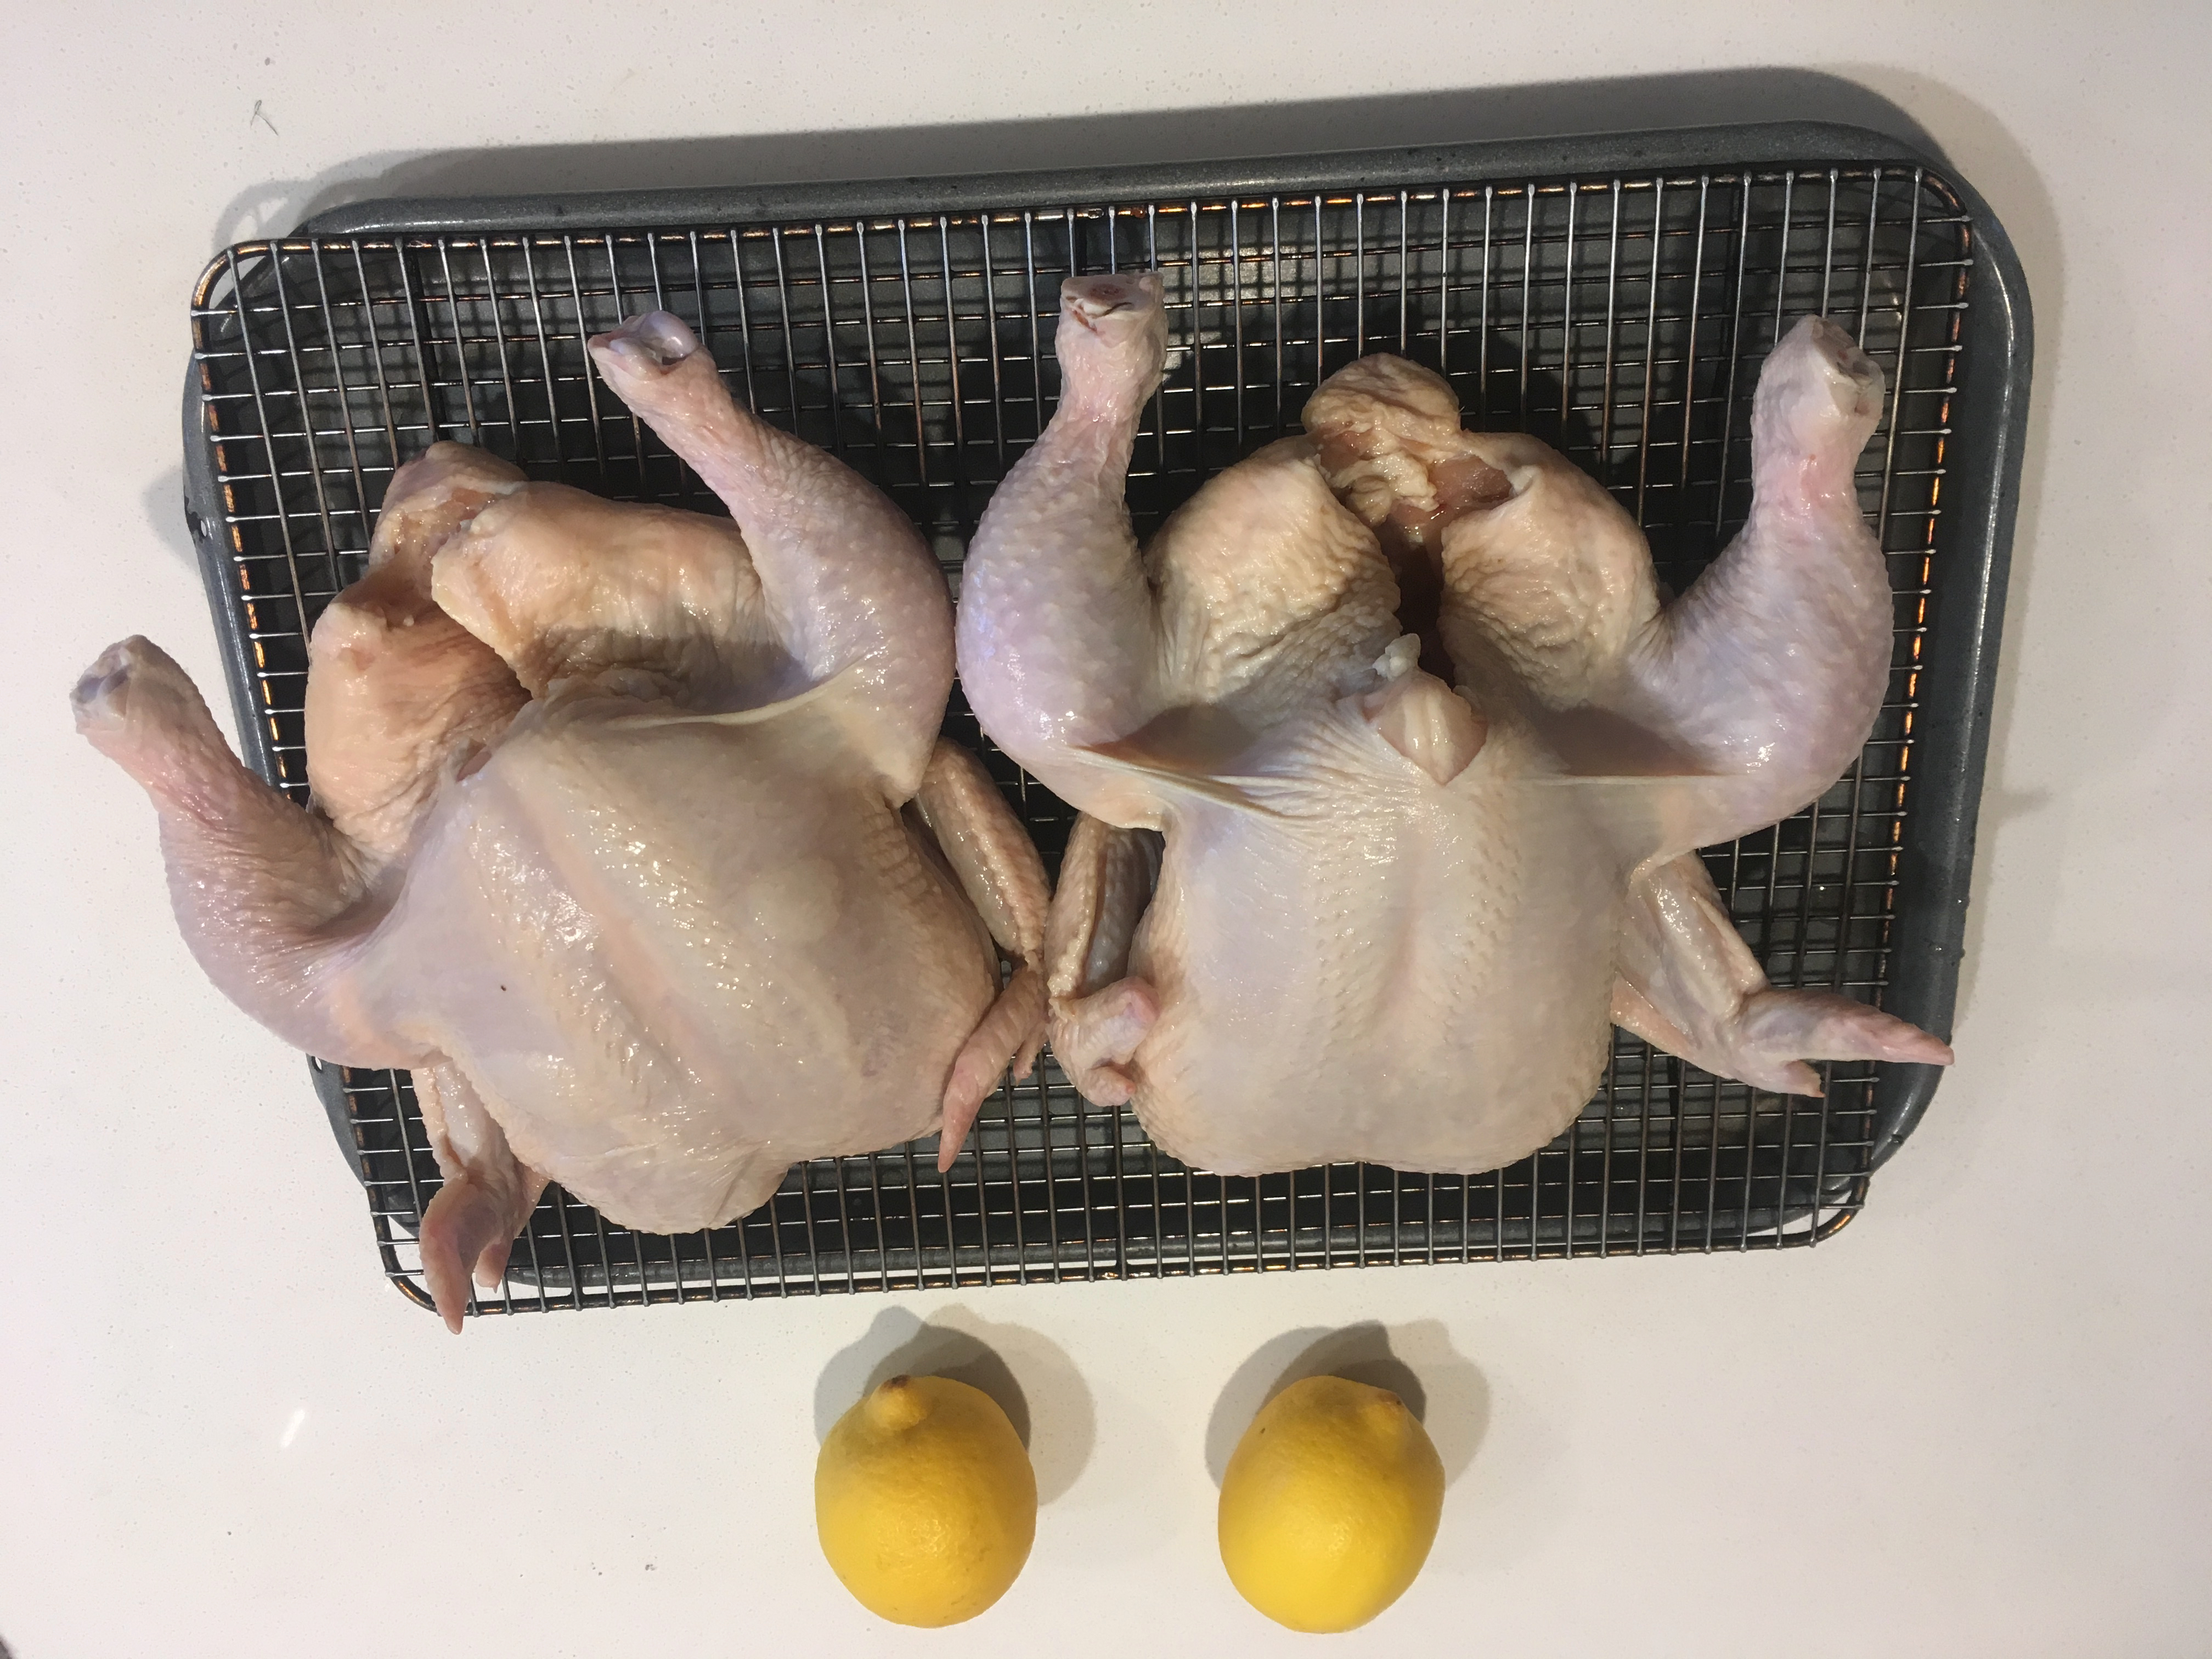
\includegraphics[width=0.25\textwidth]{\imageDir/\fileName/IMG_3197.jpg} &
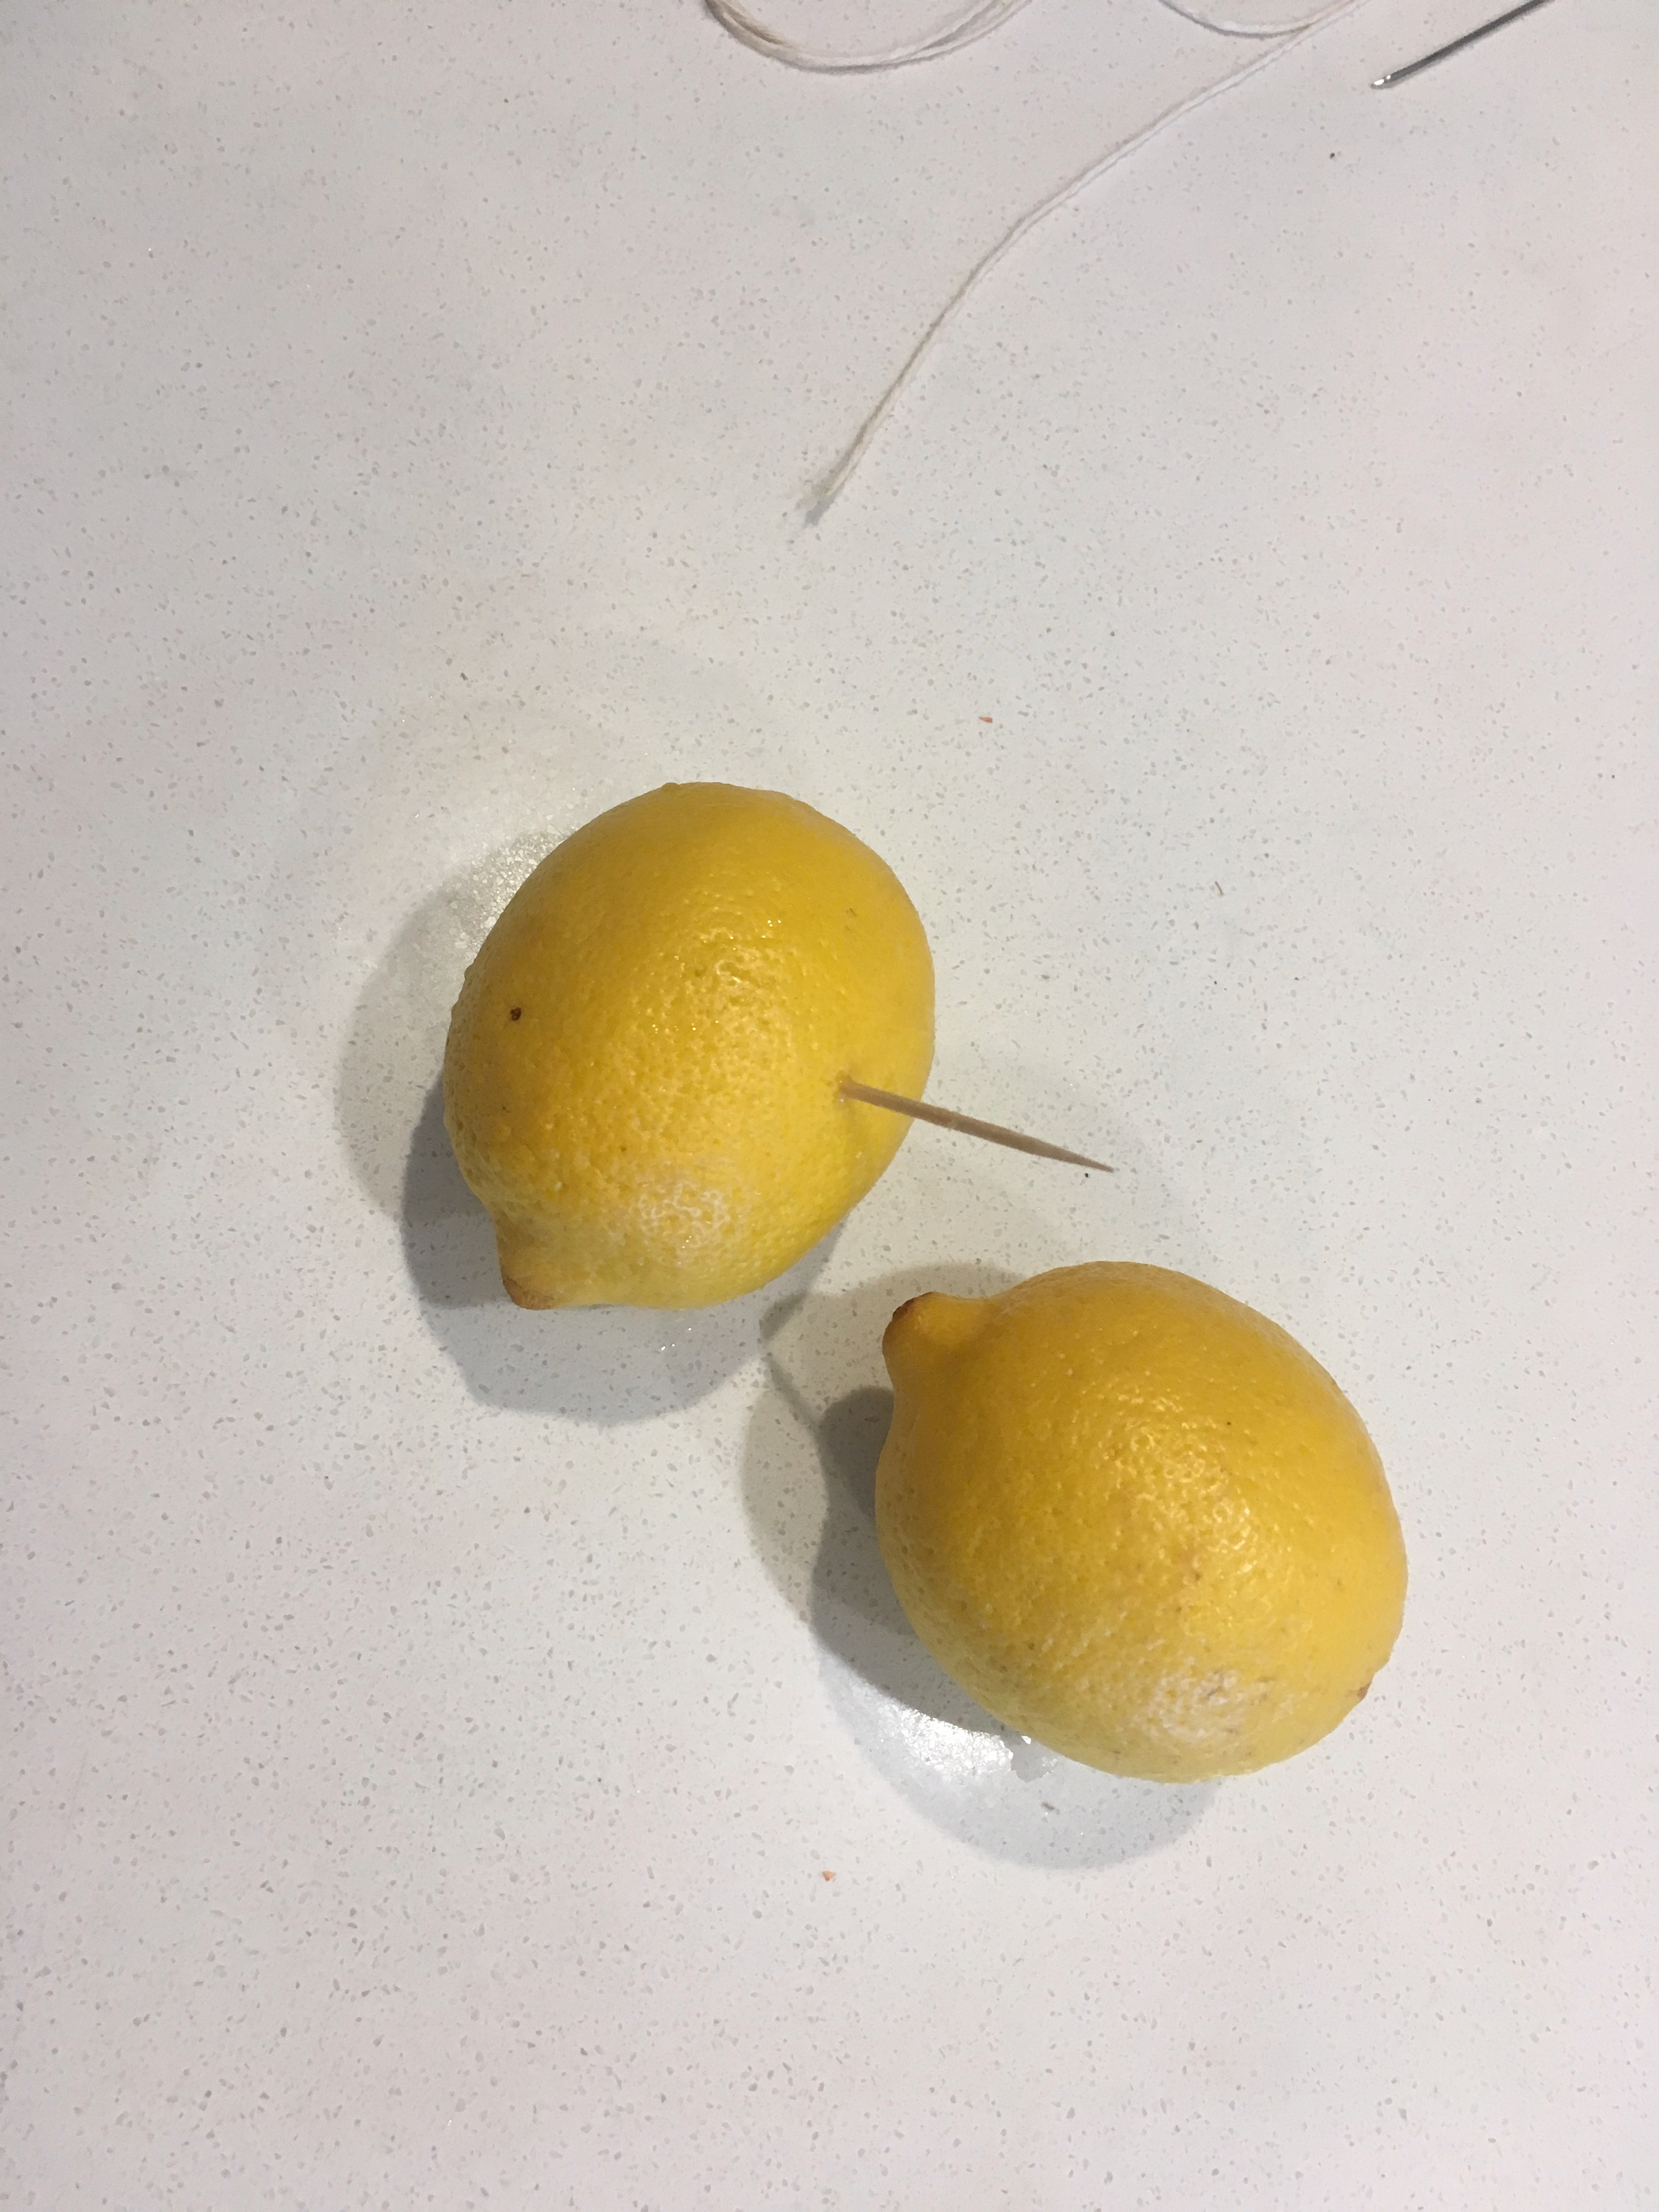
\includegraphics[width=0.25\textwidth]{\imageDir/\fileName/IMG_3212.jpg} &
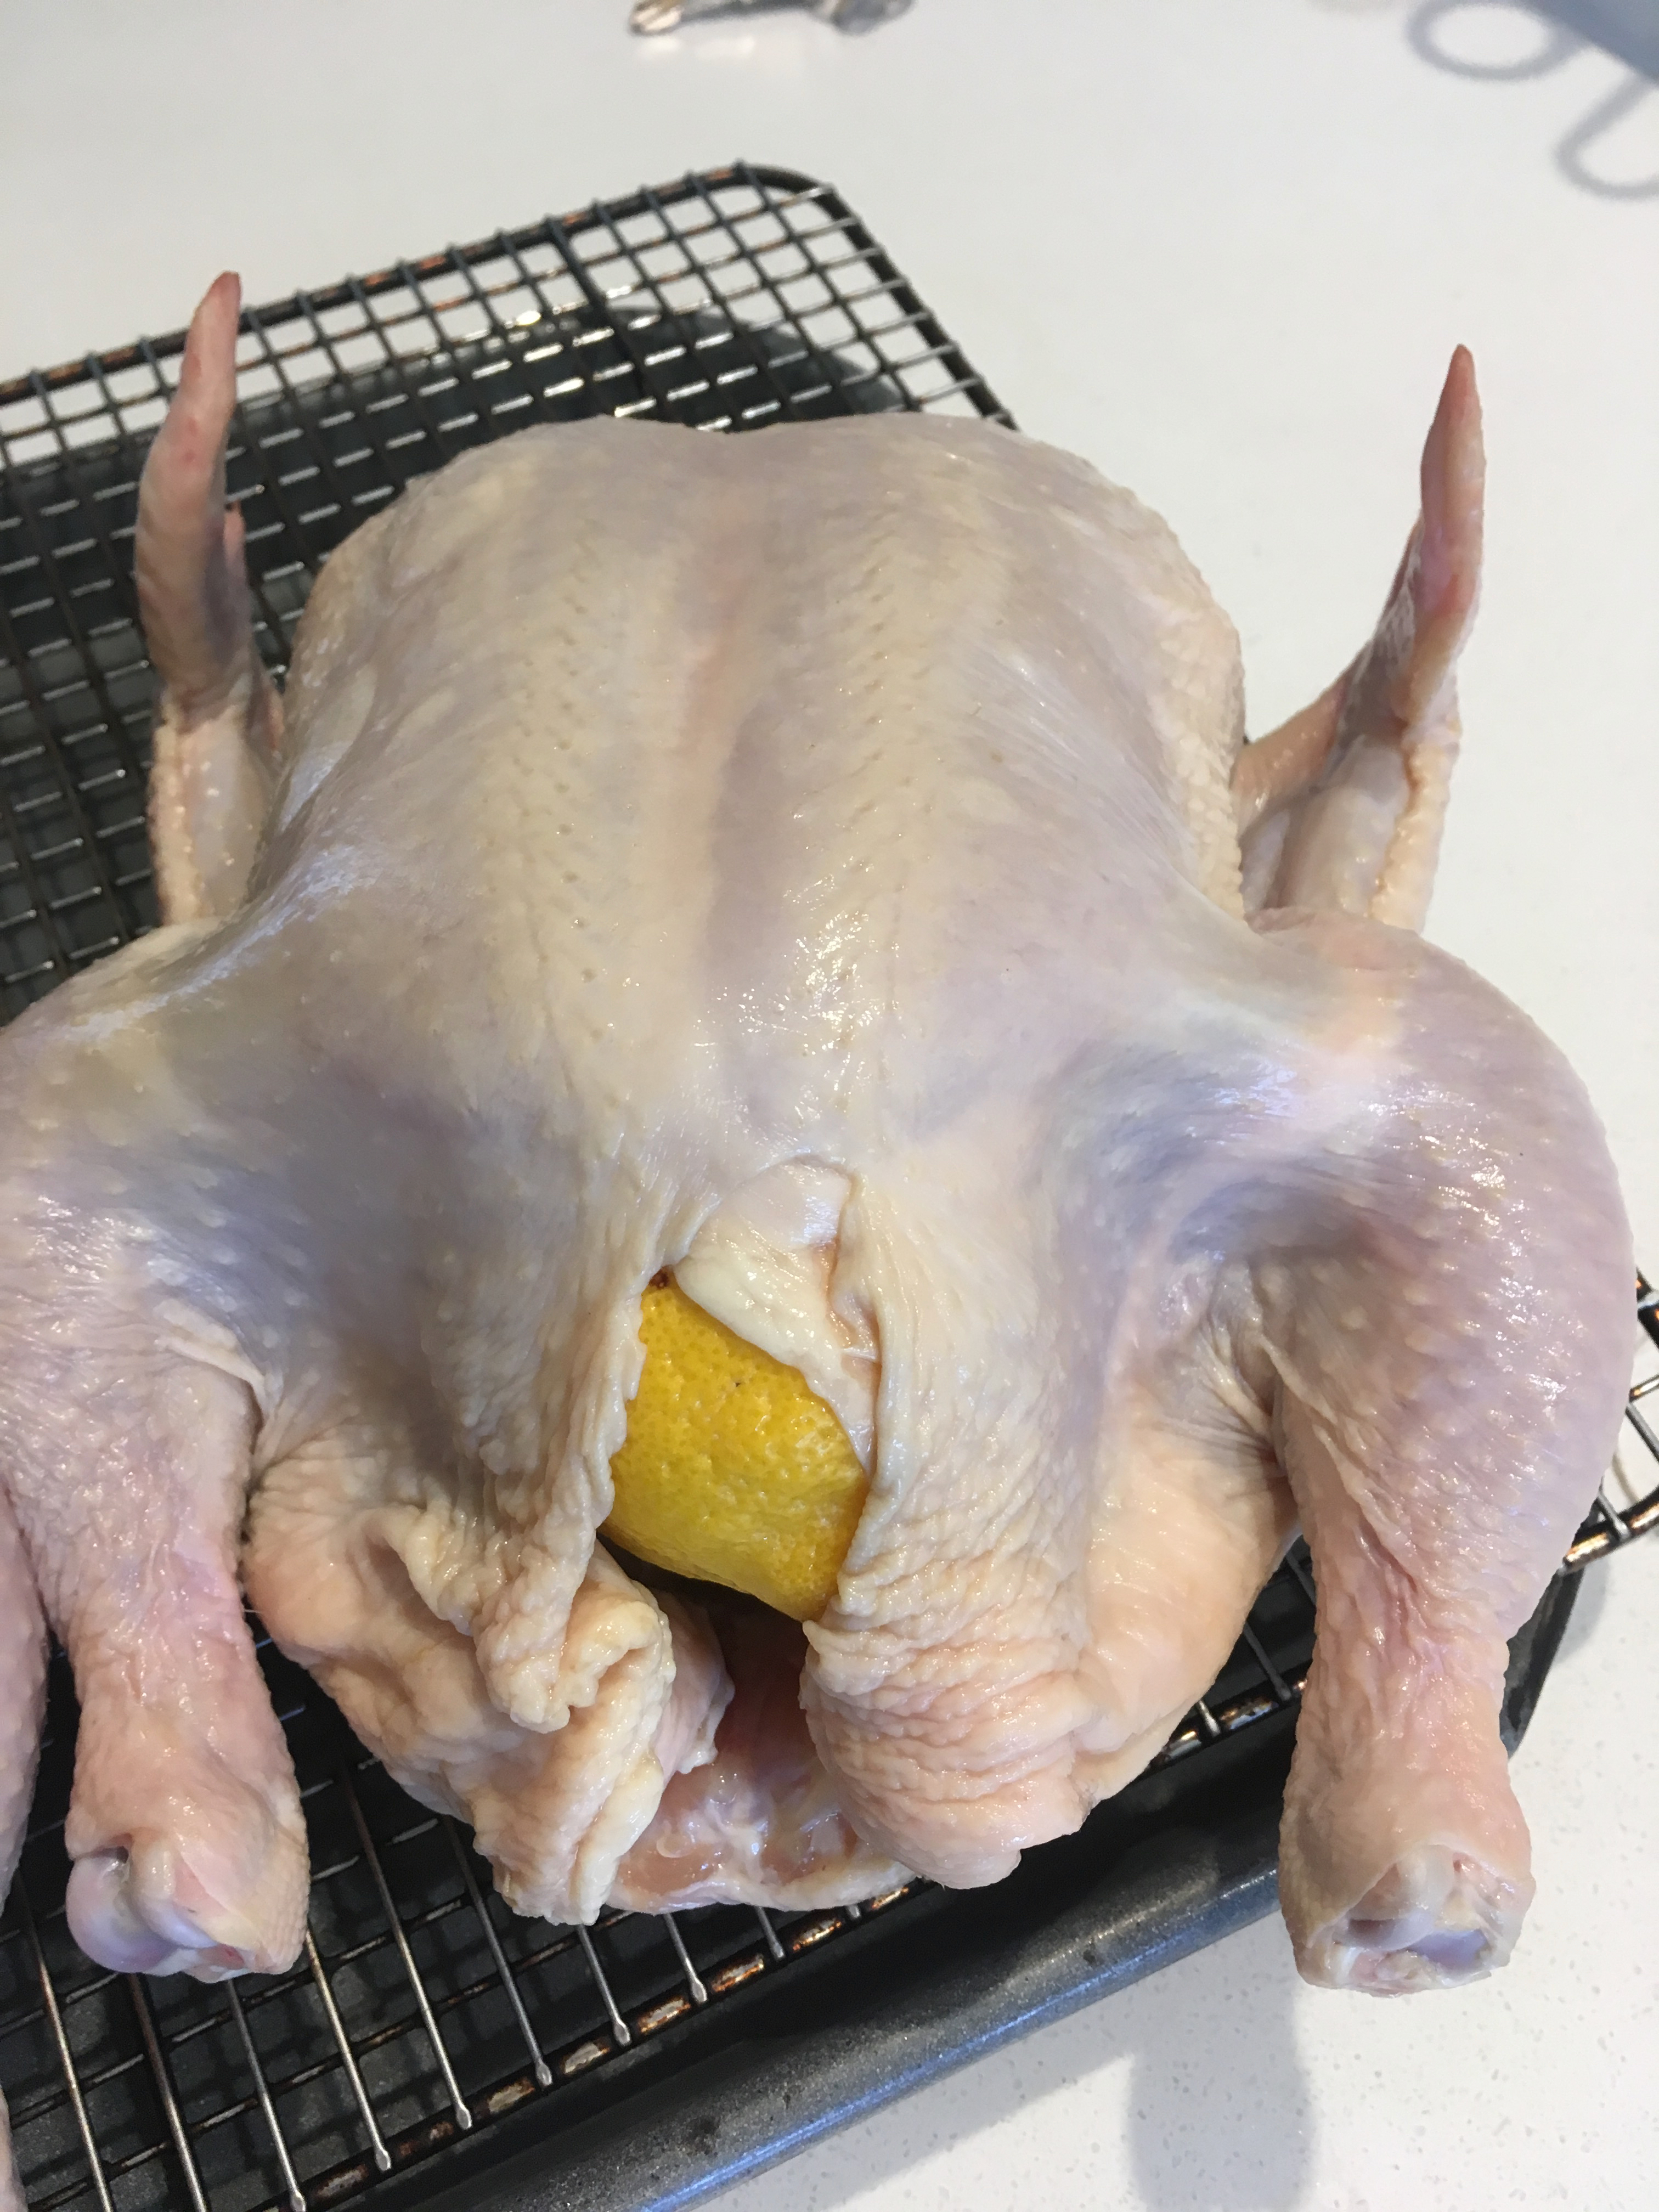
\includegraphics[width=0.25\textwidth]{\imageDir/\fileName/IMG_3213.jpg} \\
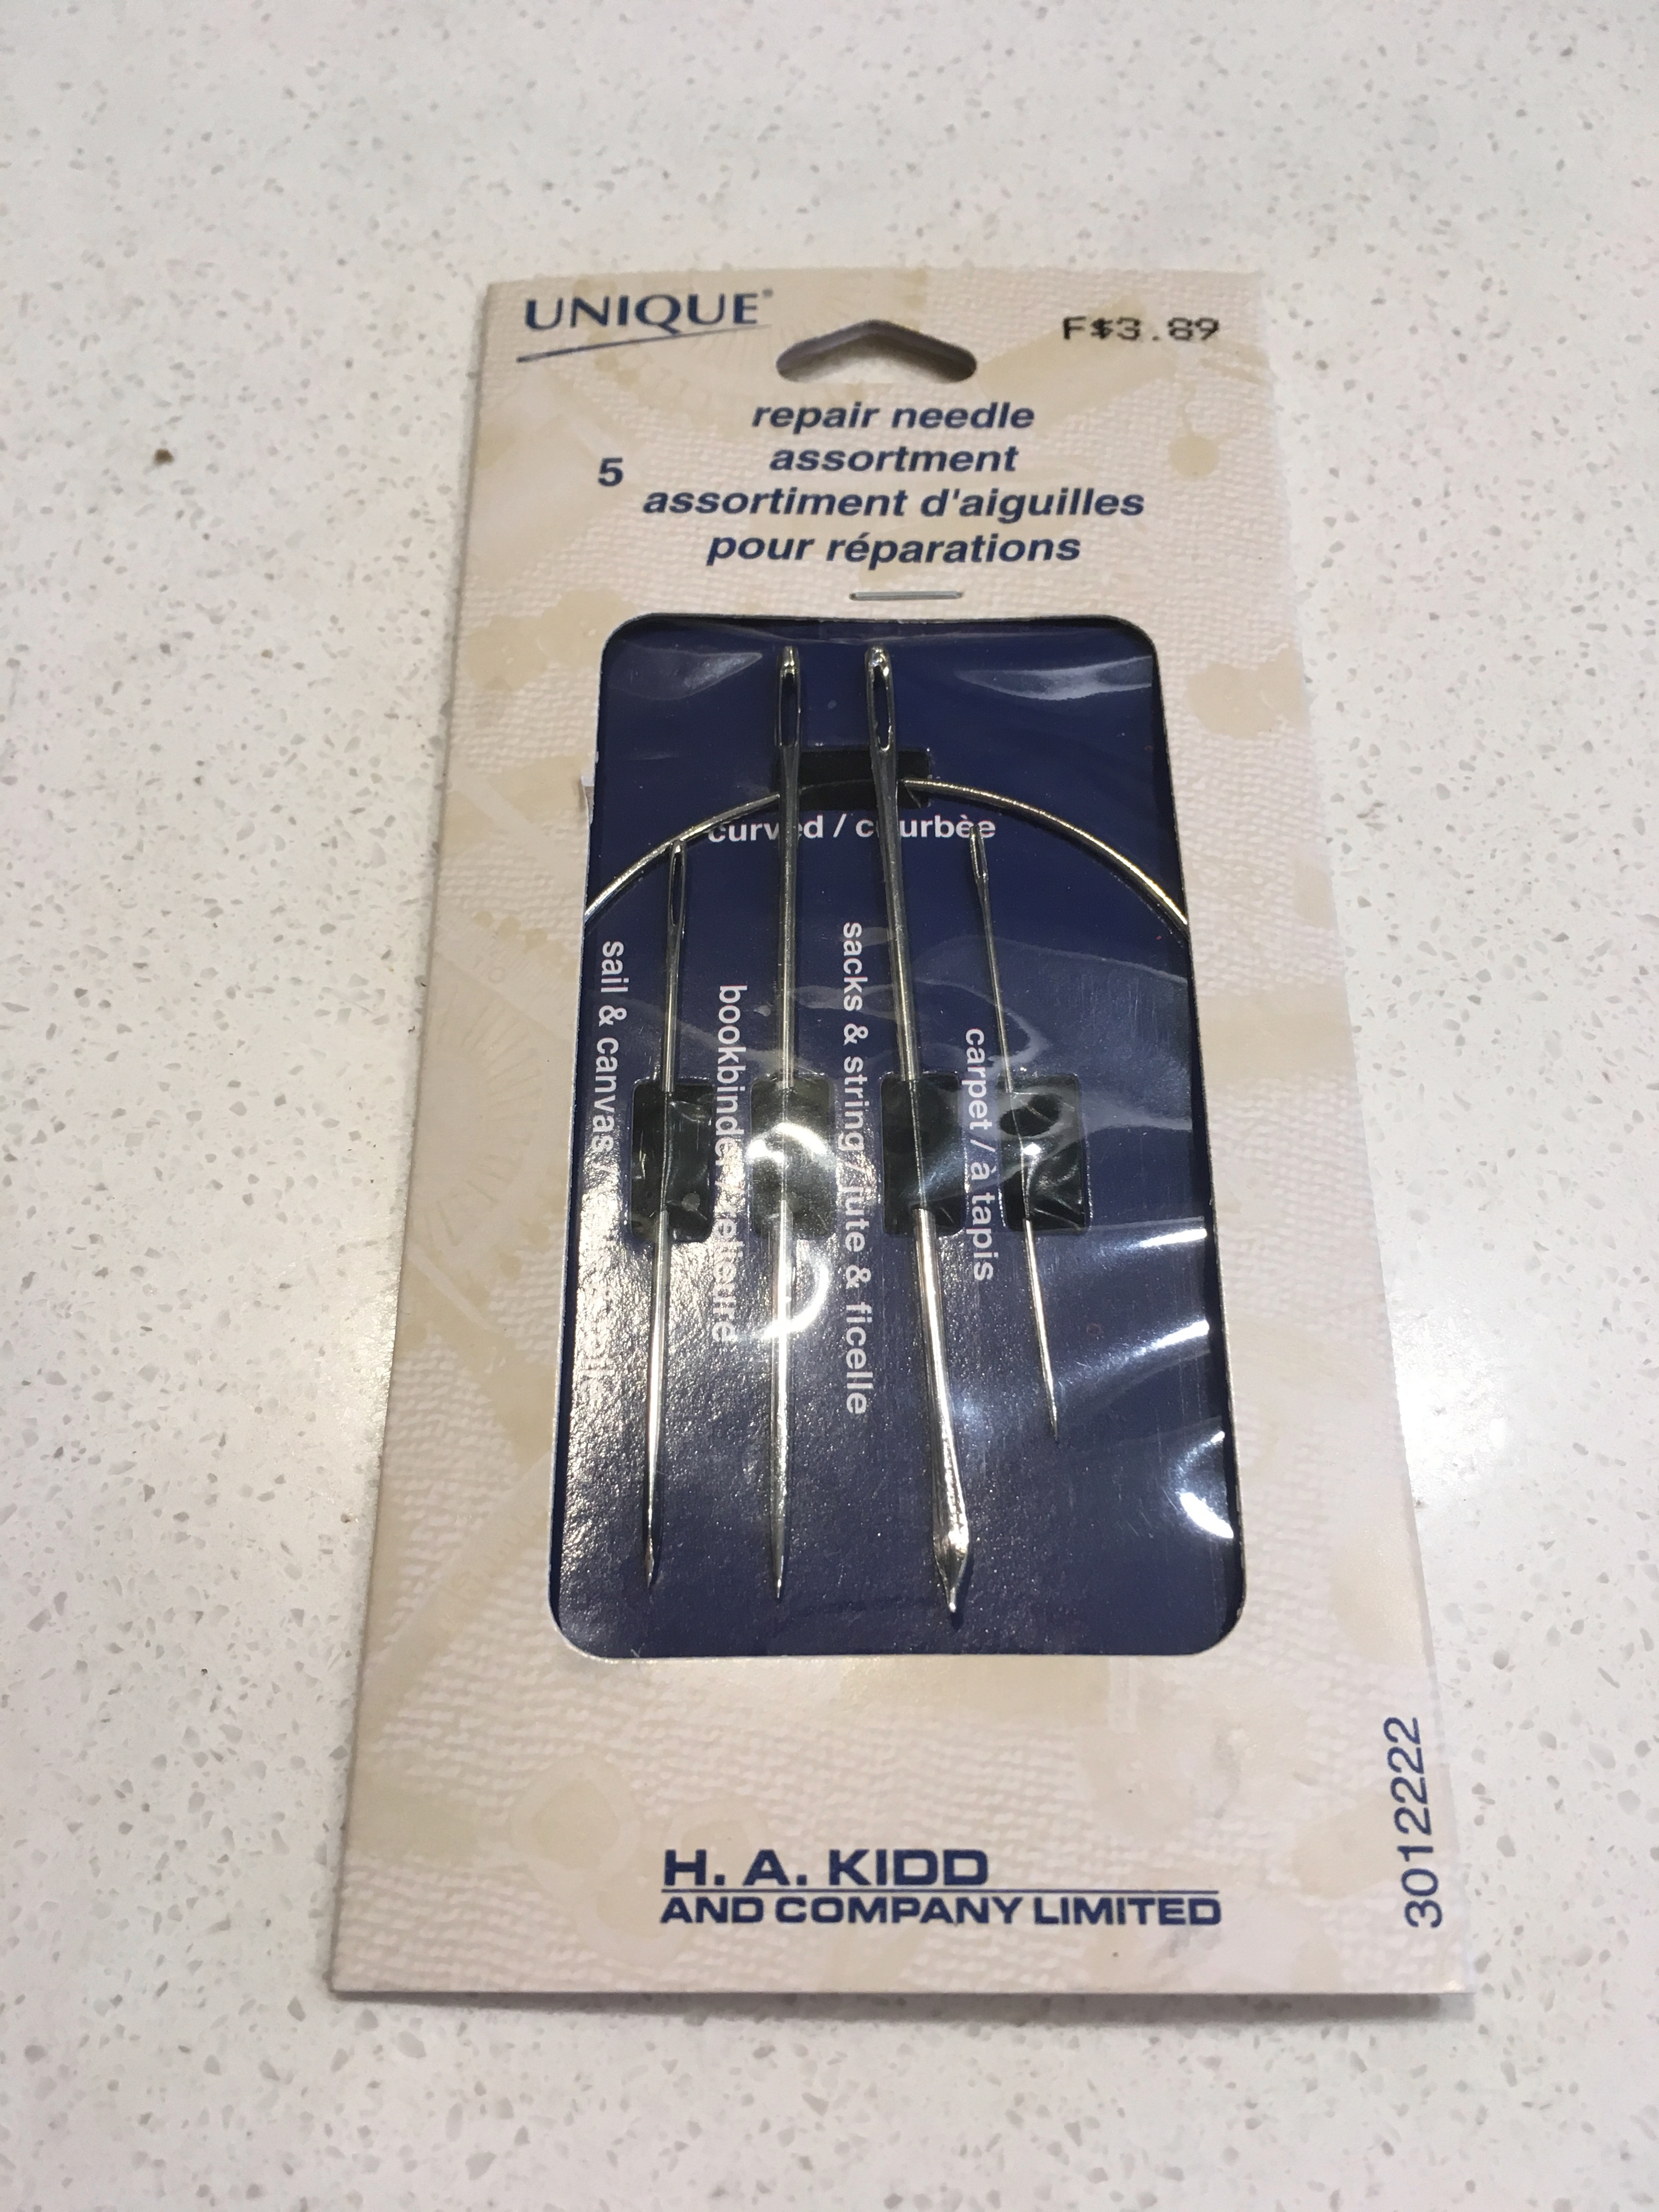
\includegraphics[width=0.25\textwidth]{\imageDir/\fileName/IMG_3206.jpg} &
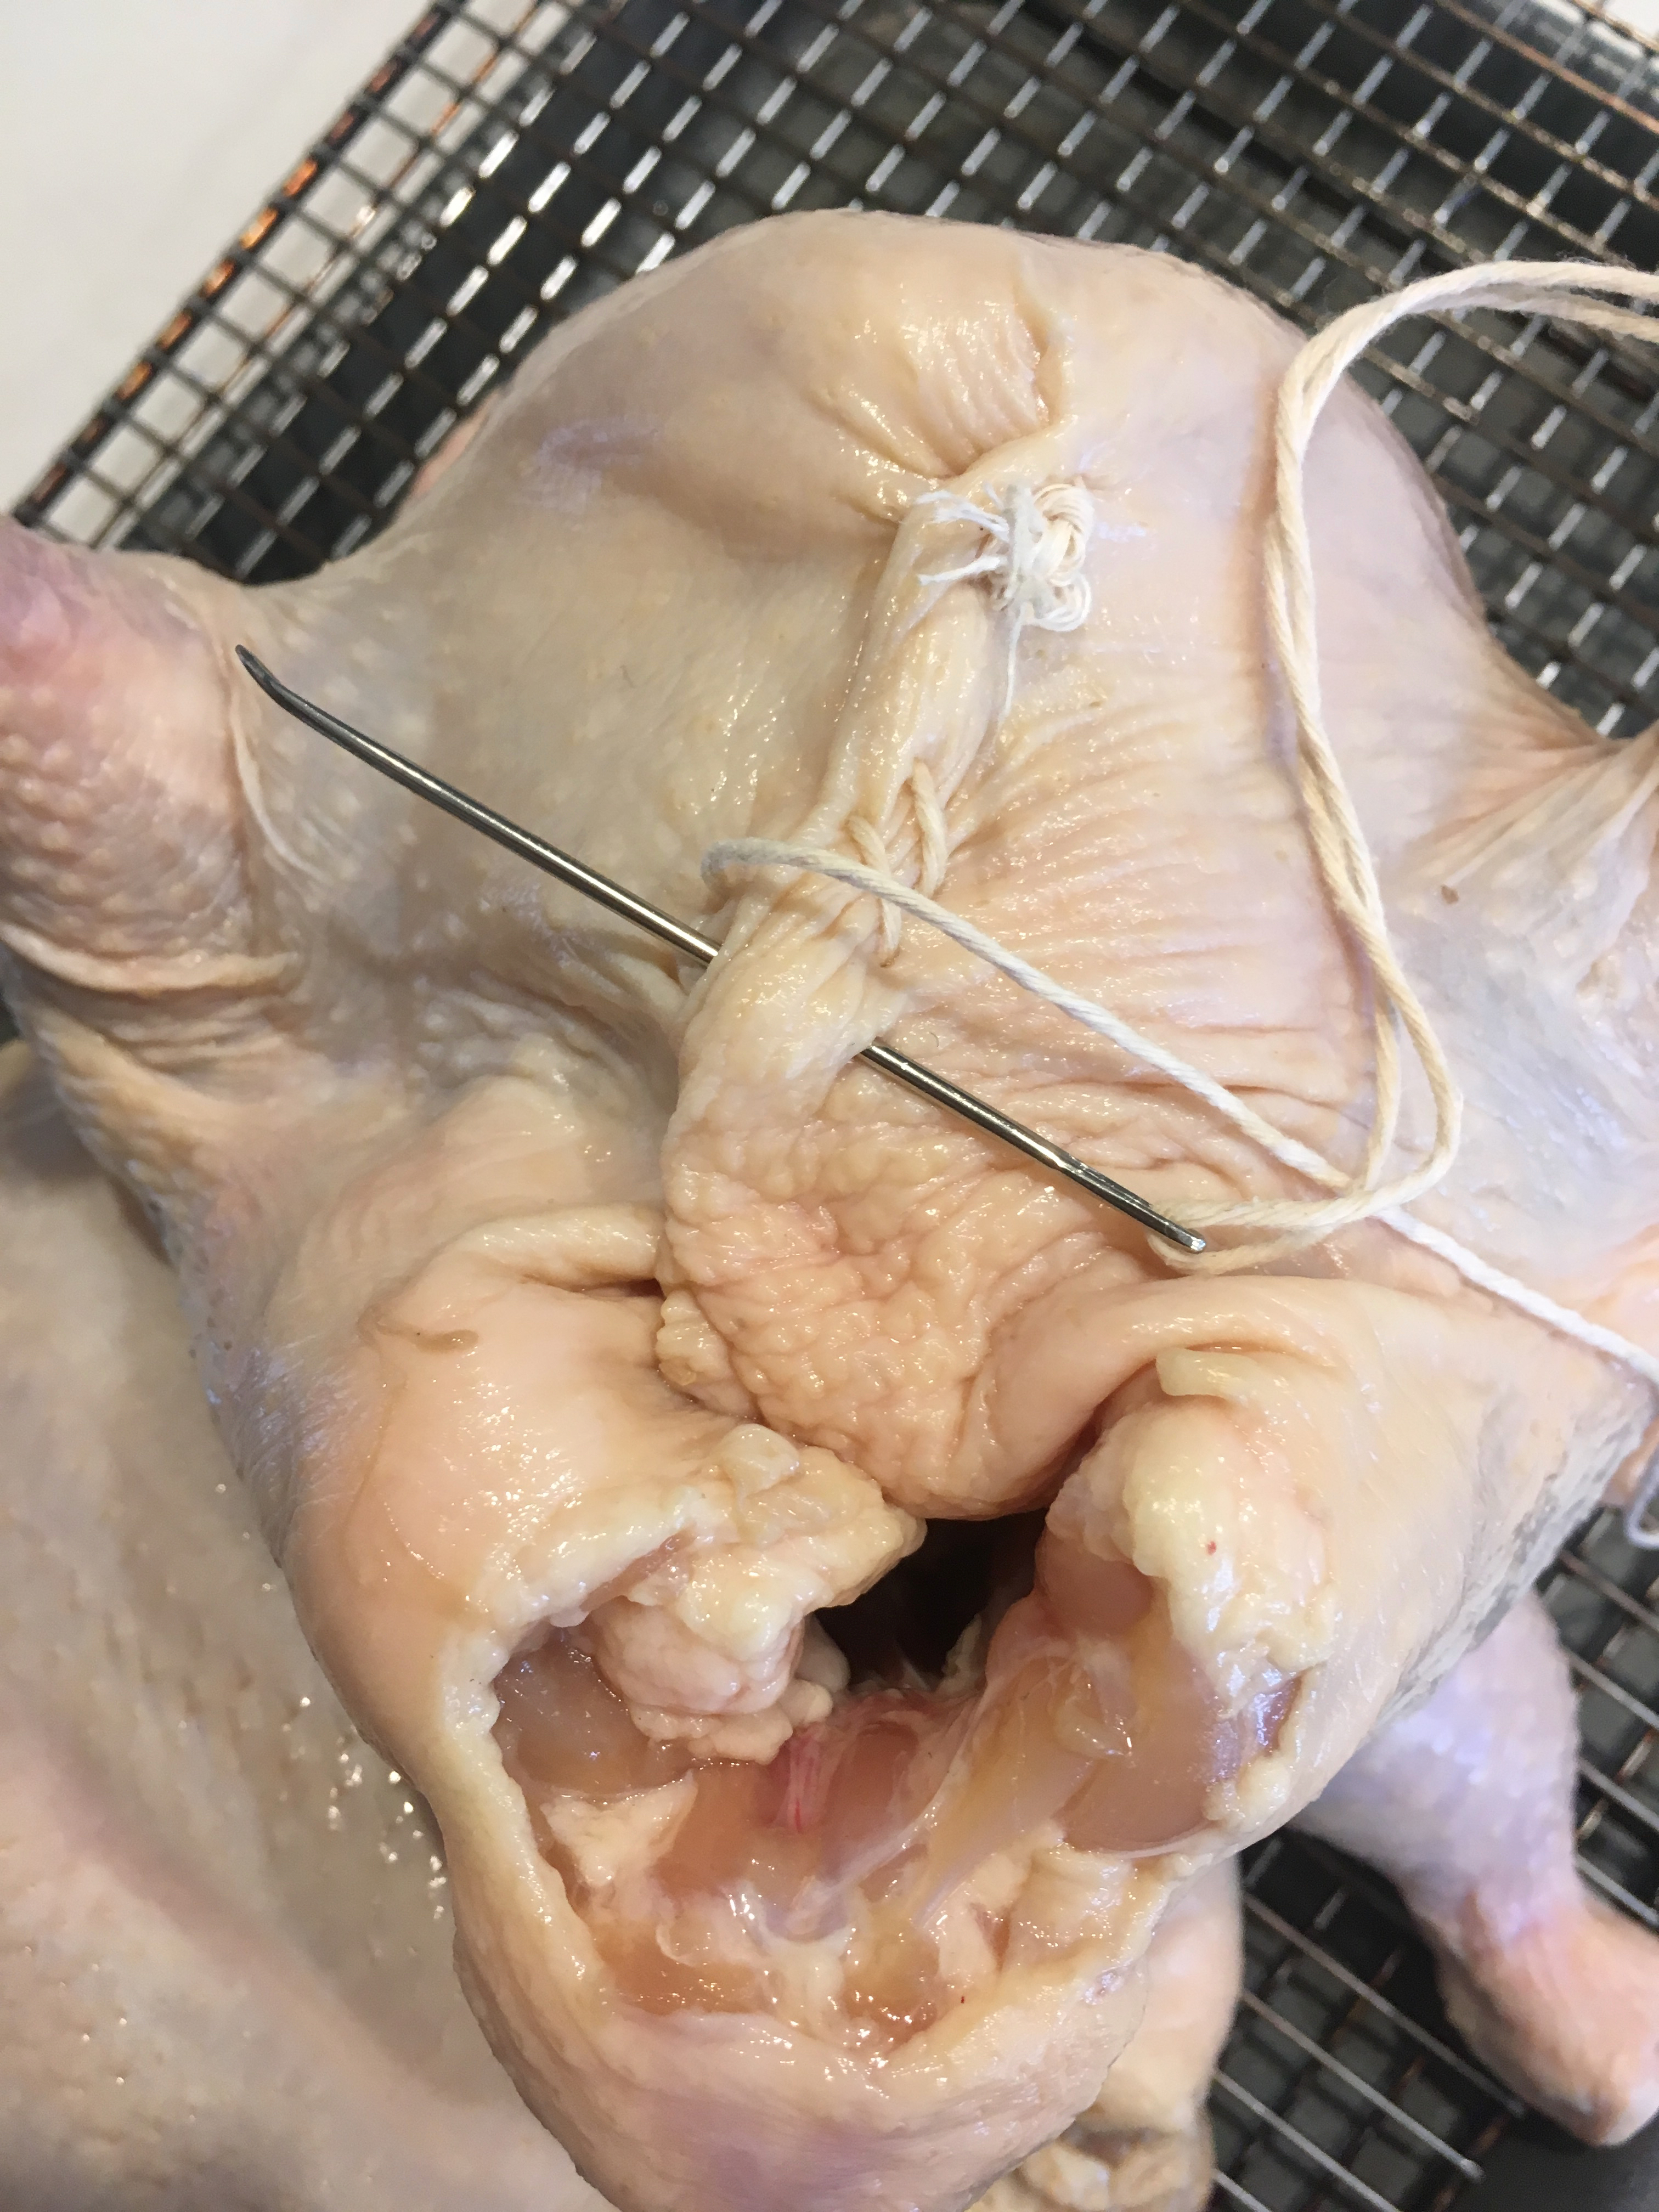
\includegraphics[width=0.25\textwidth]{\imageDir/\fileName/IMG_3214.jpg} &
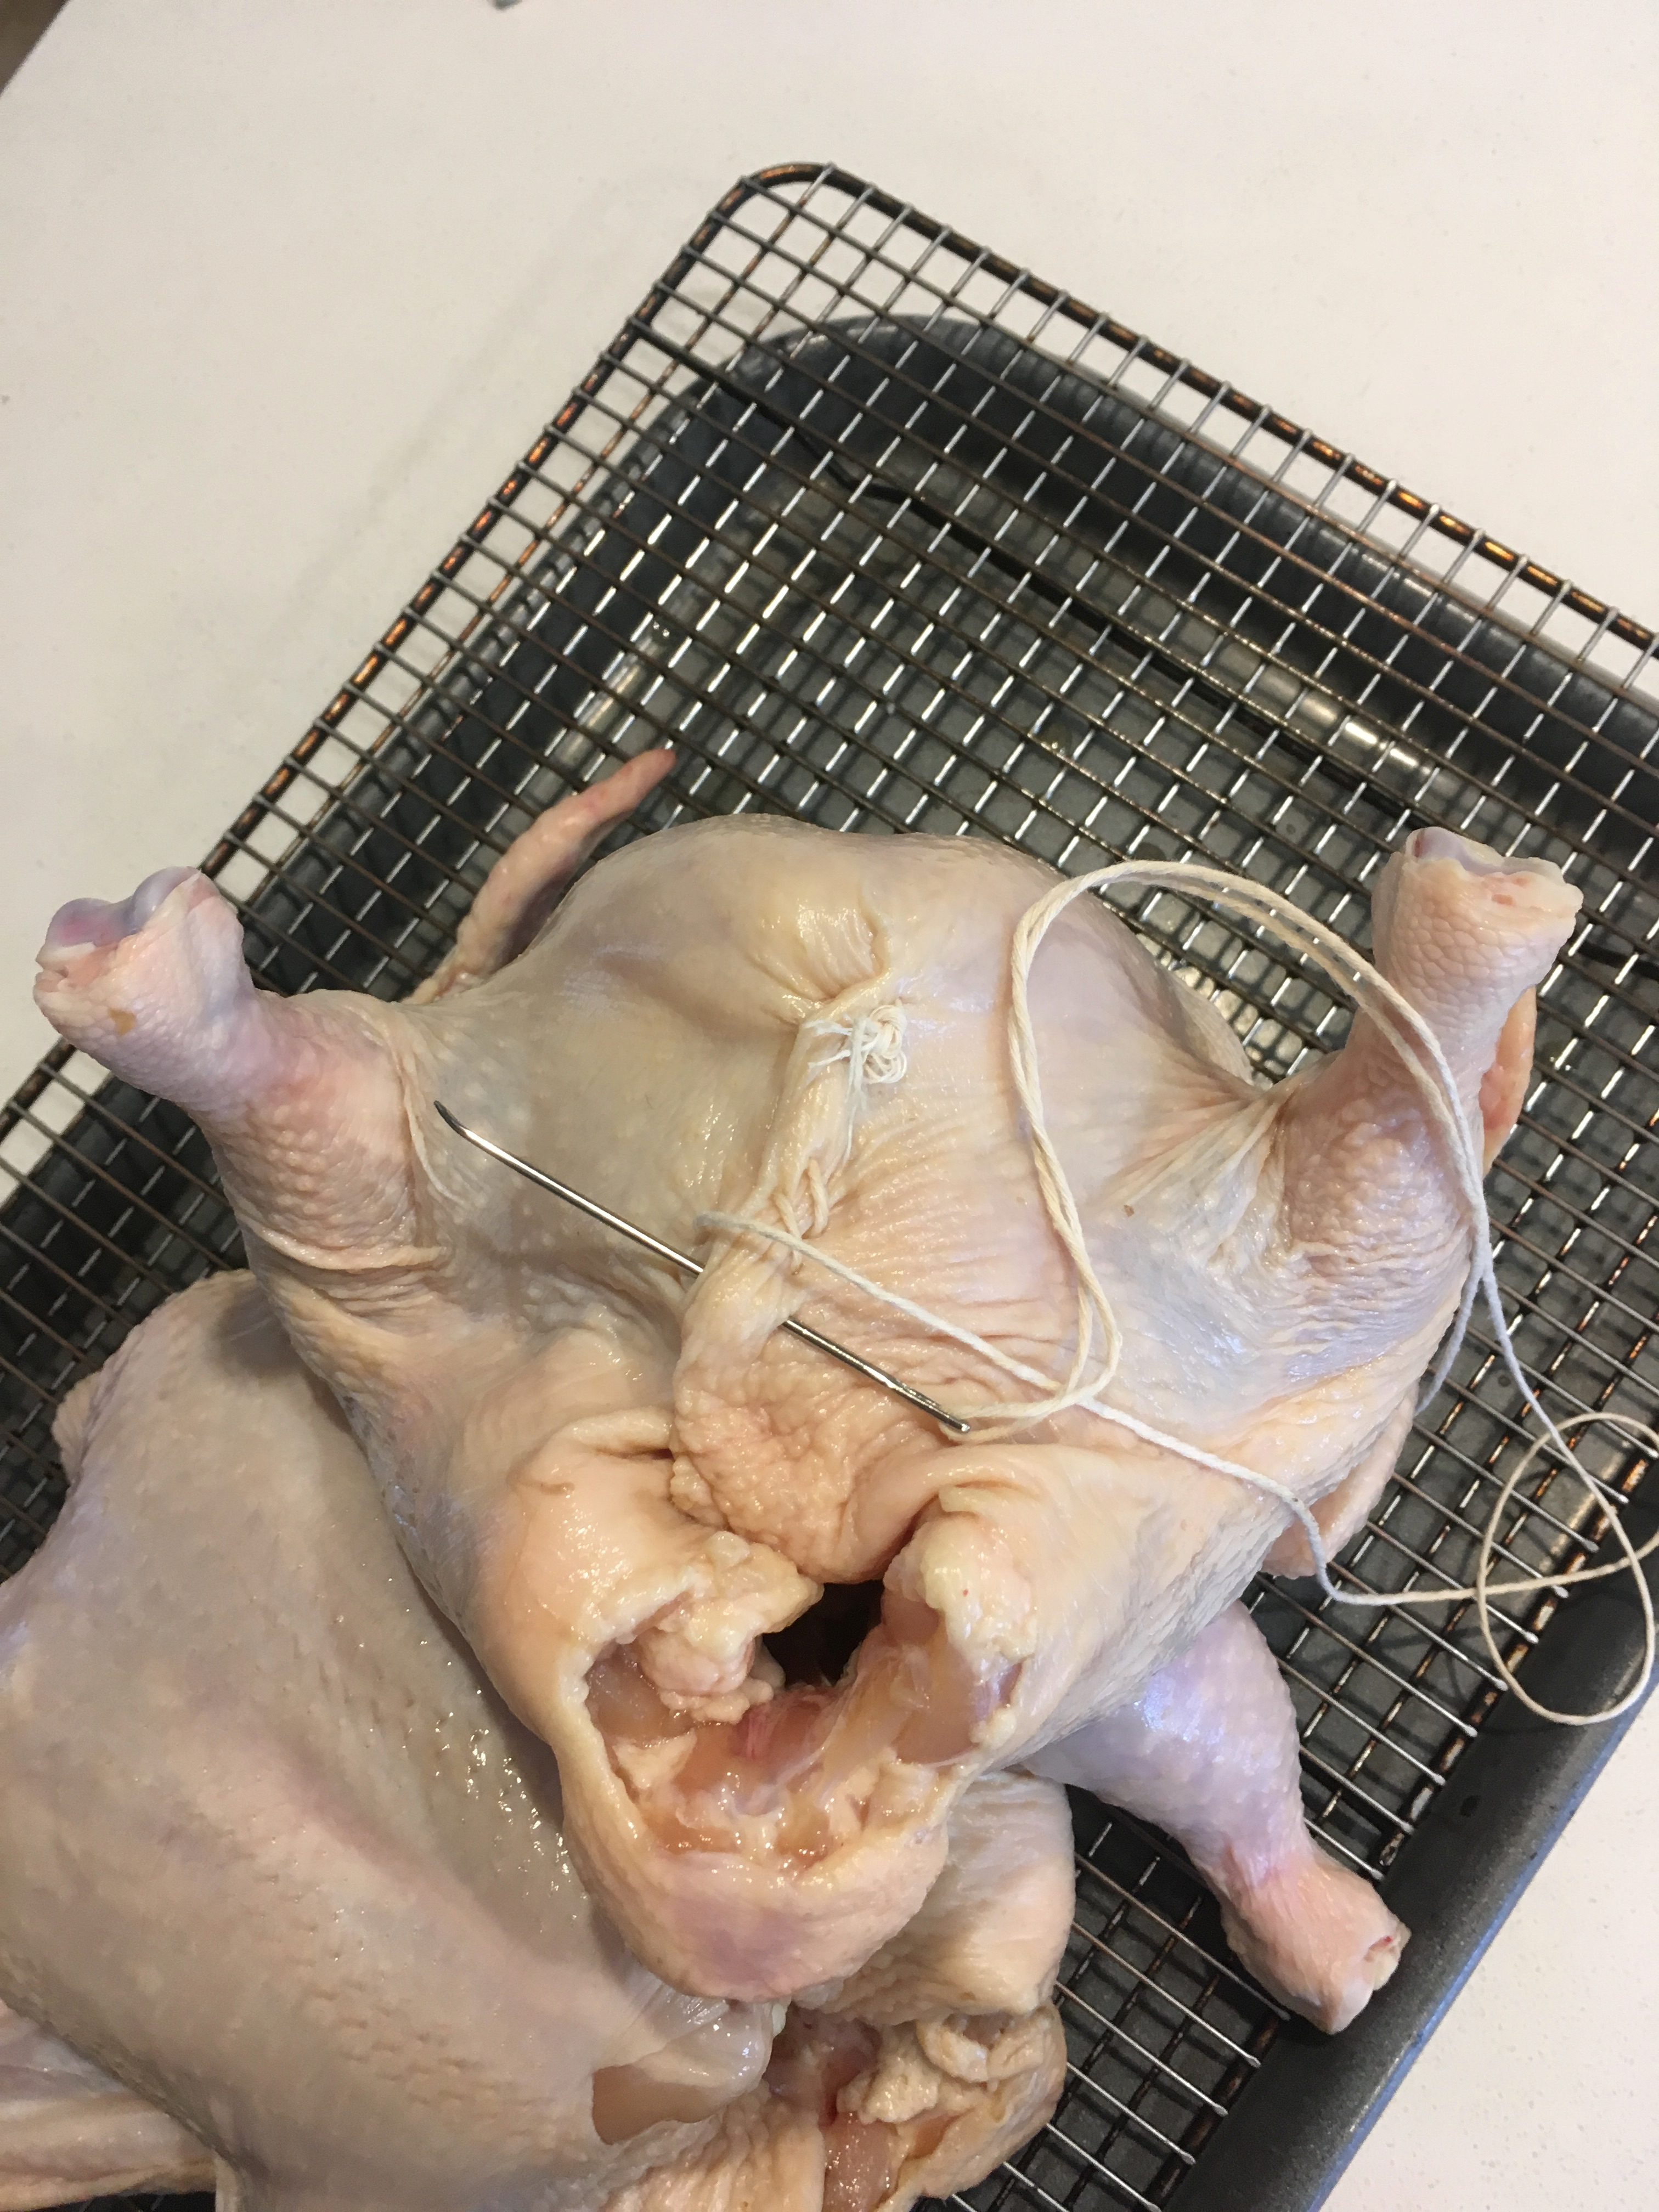
\includegraphics[width=0.25\textwidth]{\imageDir/\fileName/IMG_3216.jpg} \\
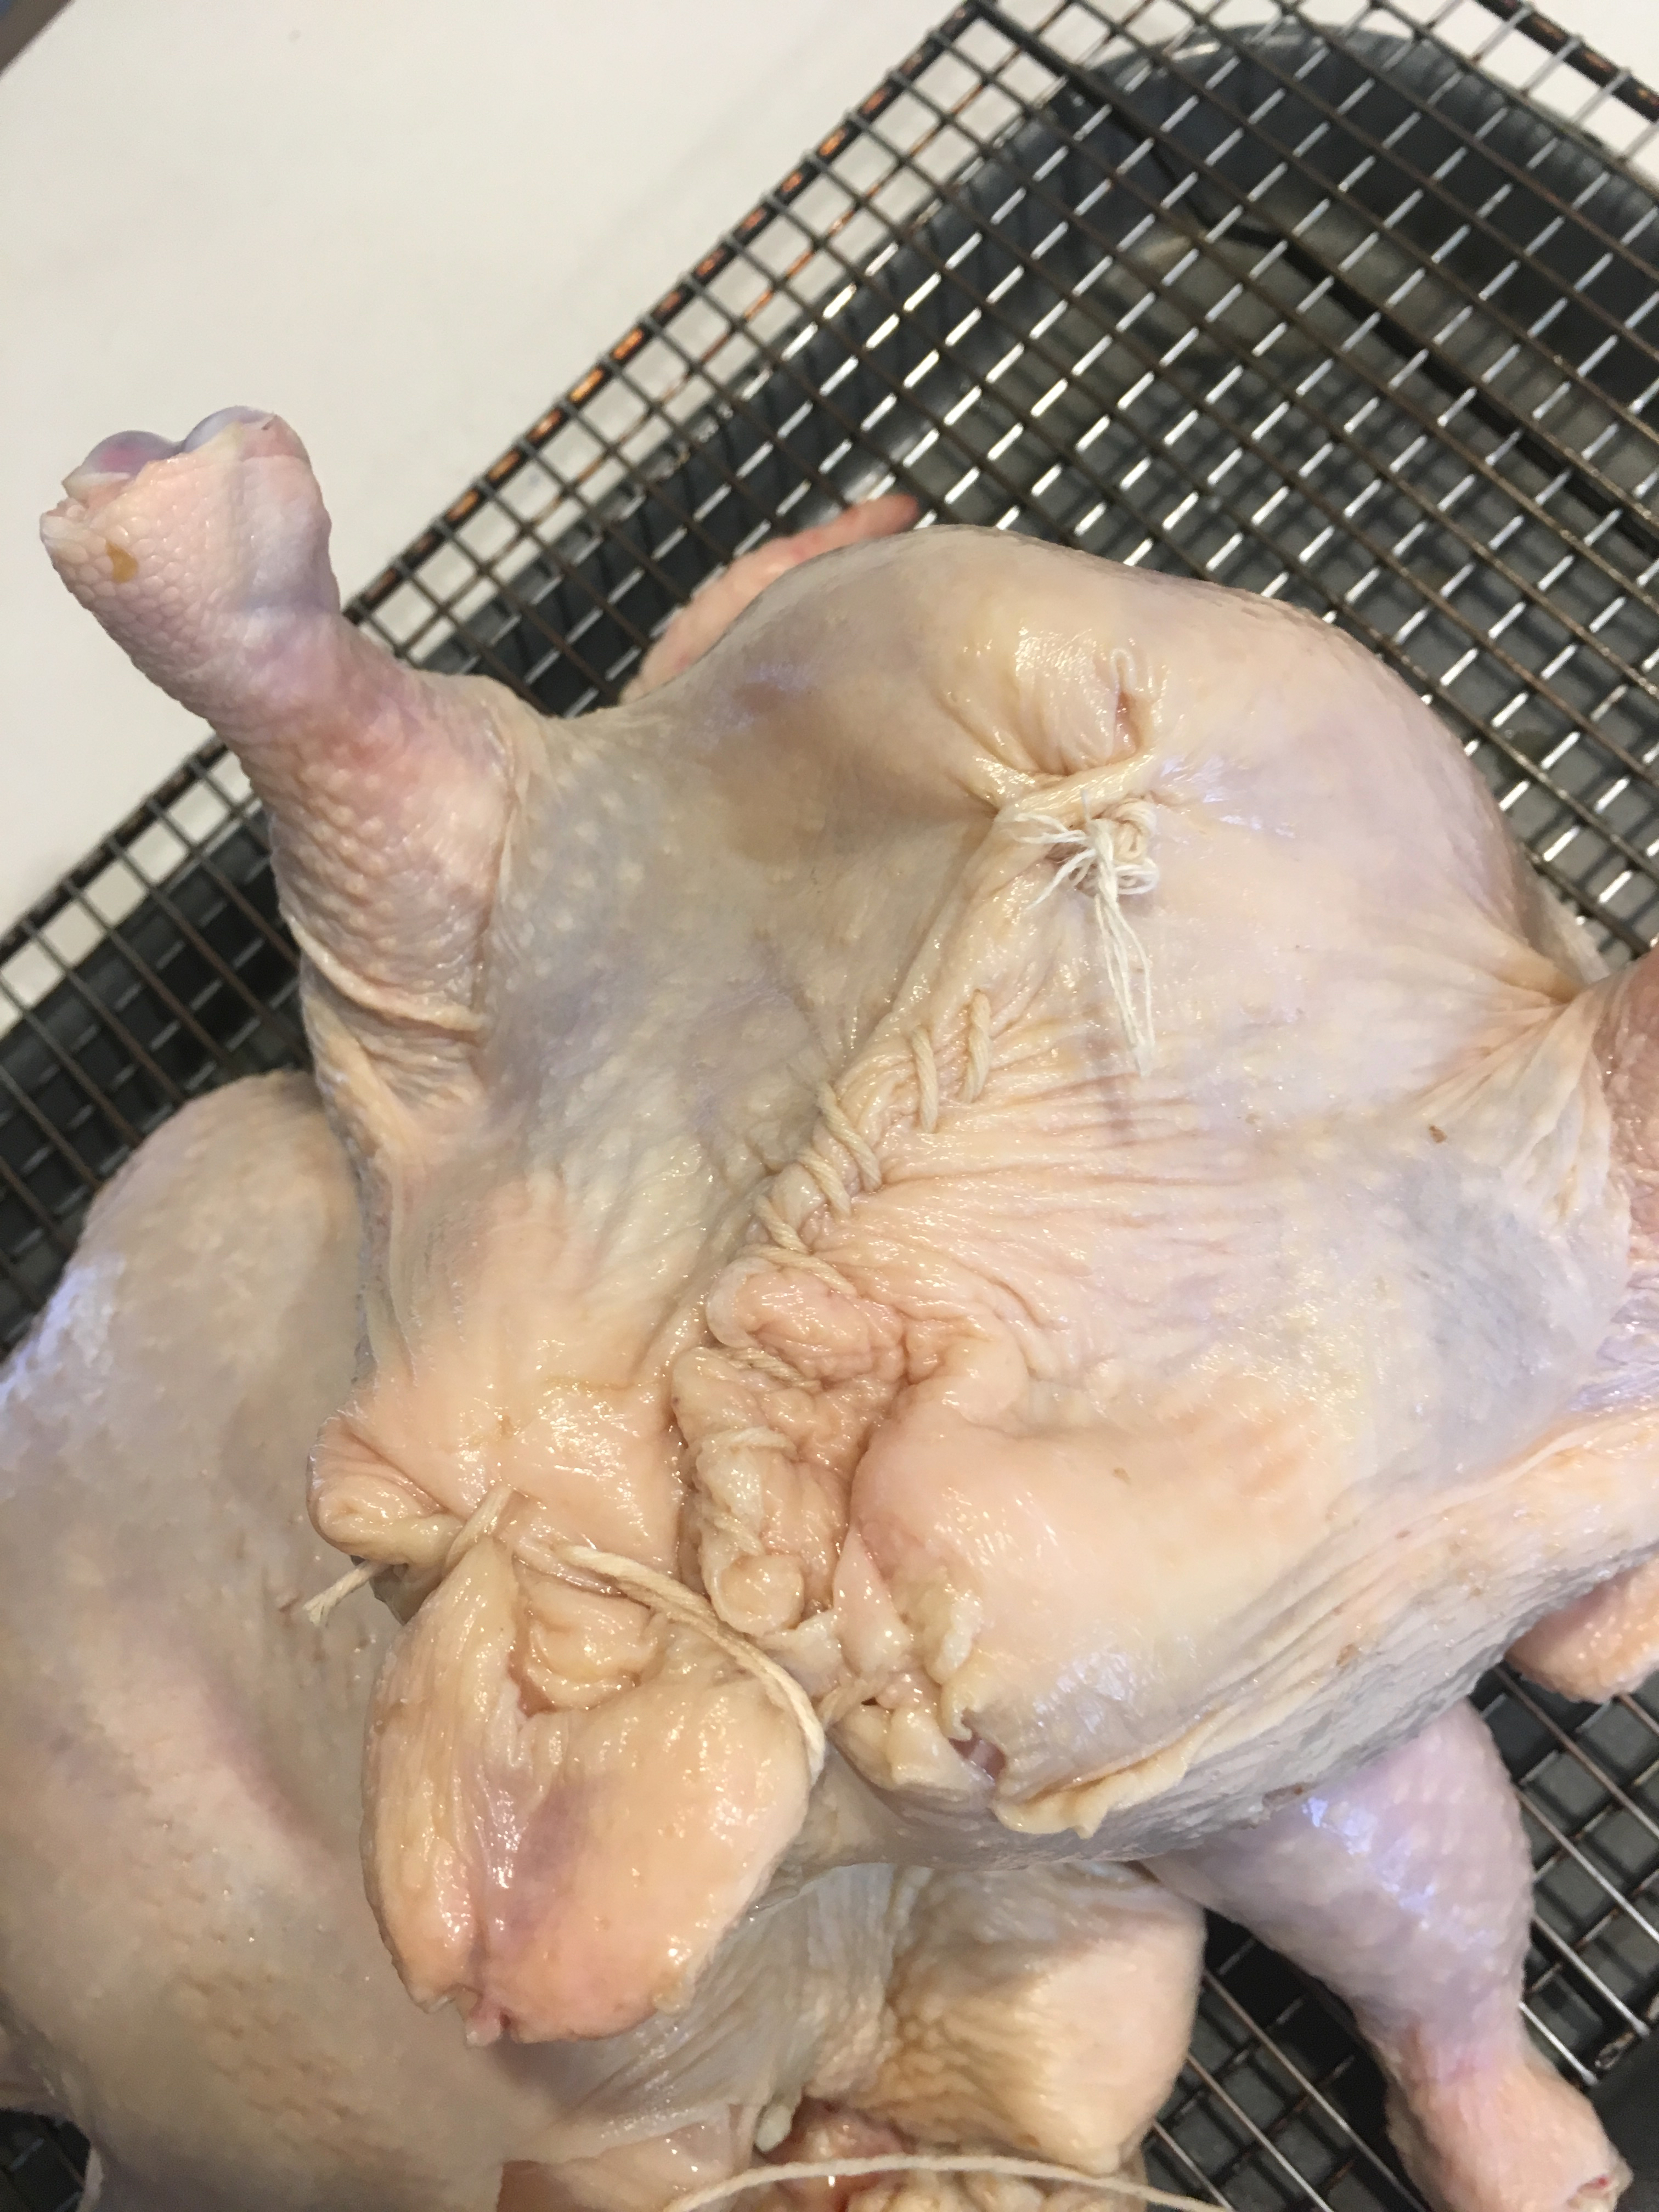
\includegraphics[width=0.25\textwidth]{\imageDir/\fileName/IMG_3217.jpg} &
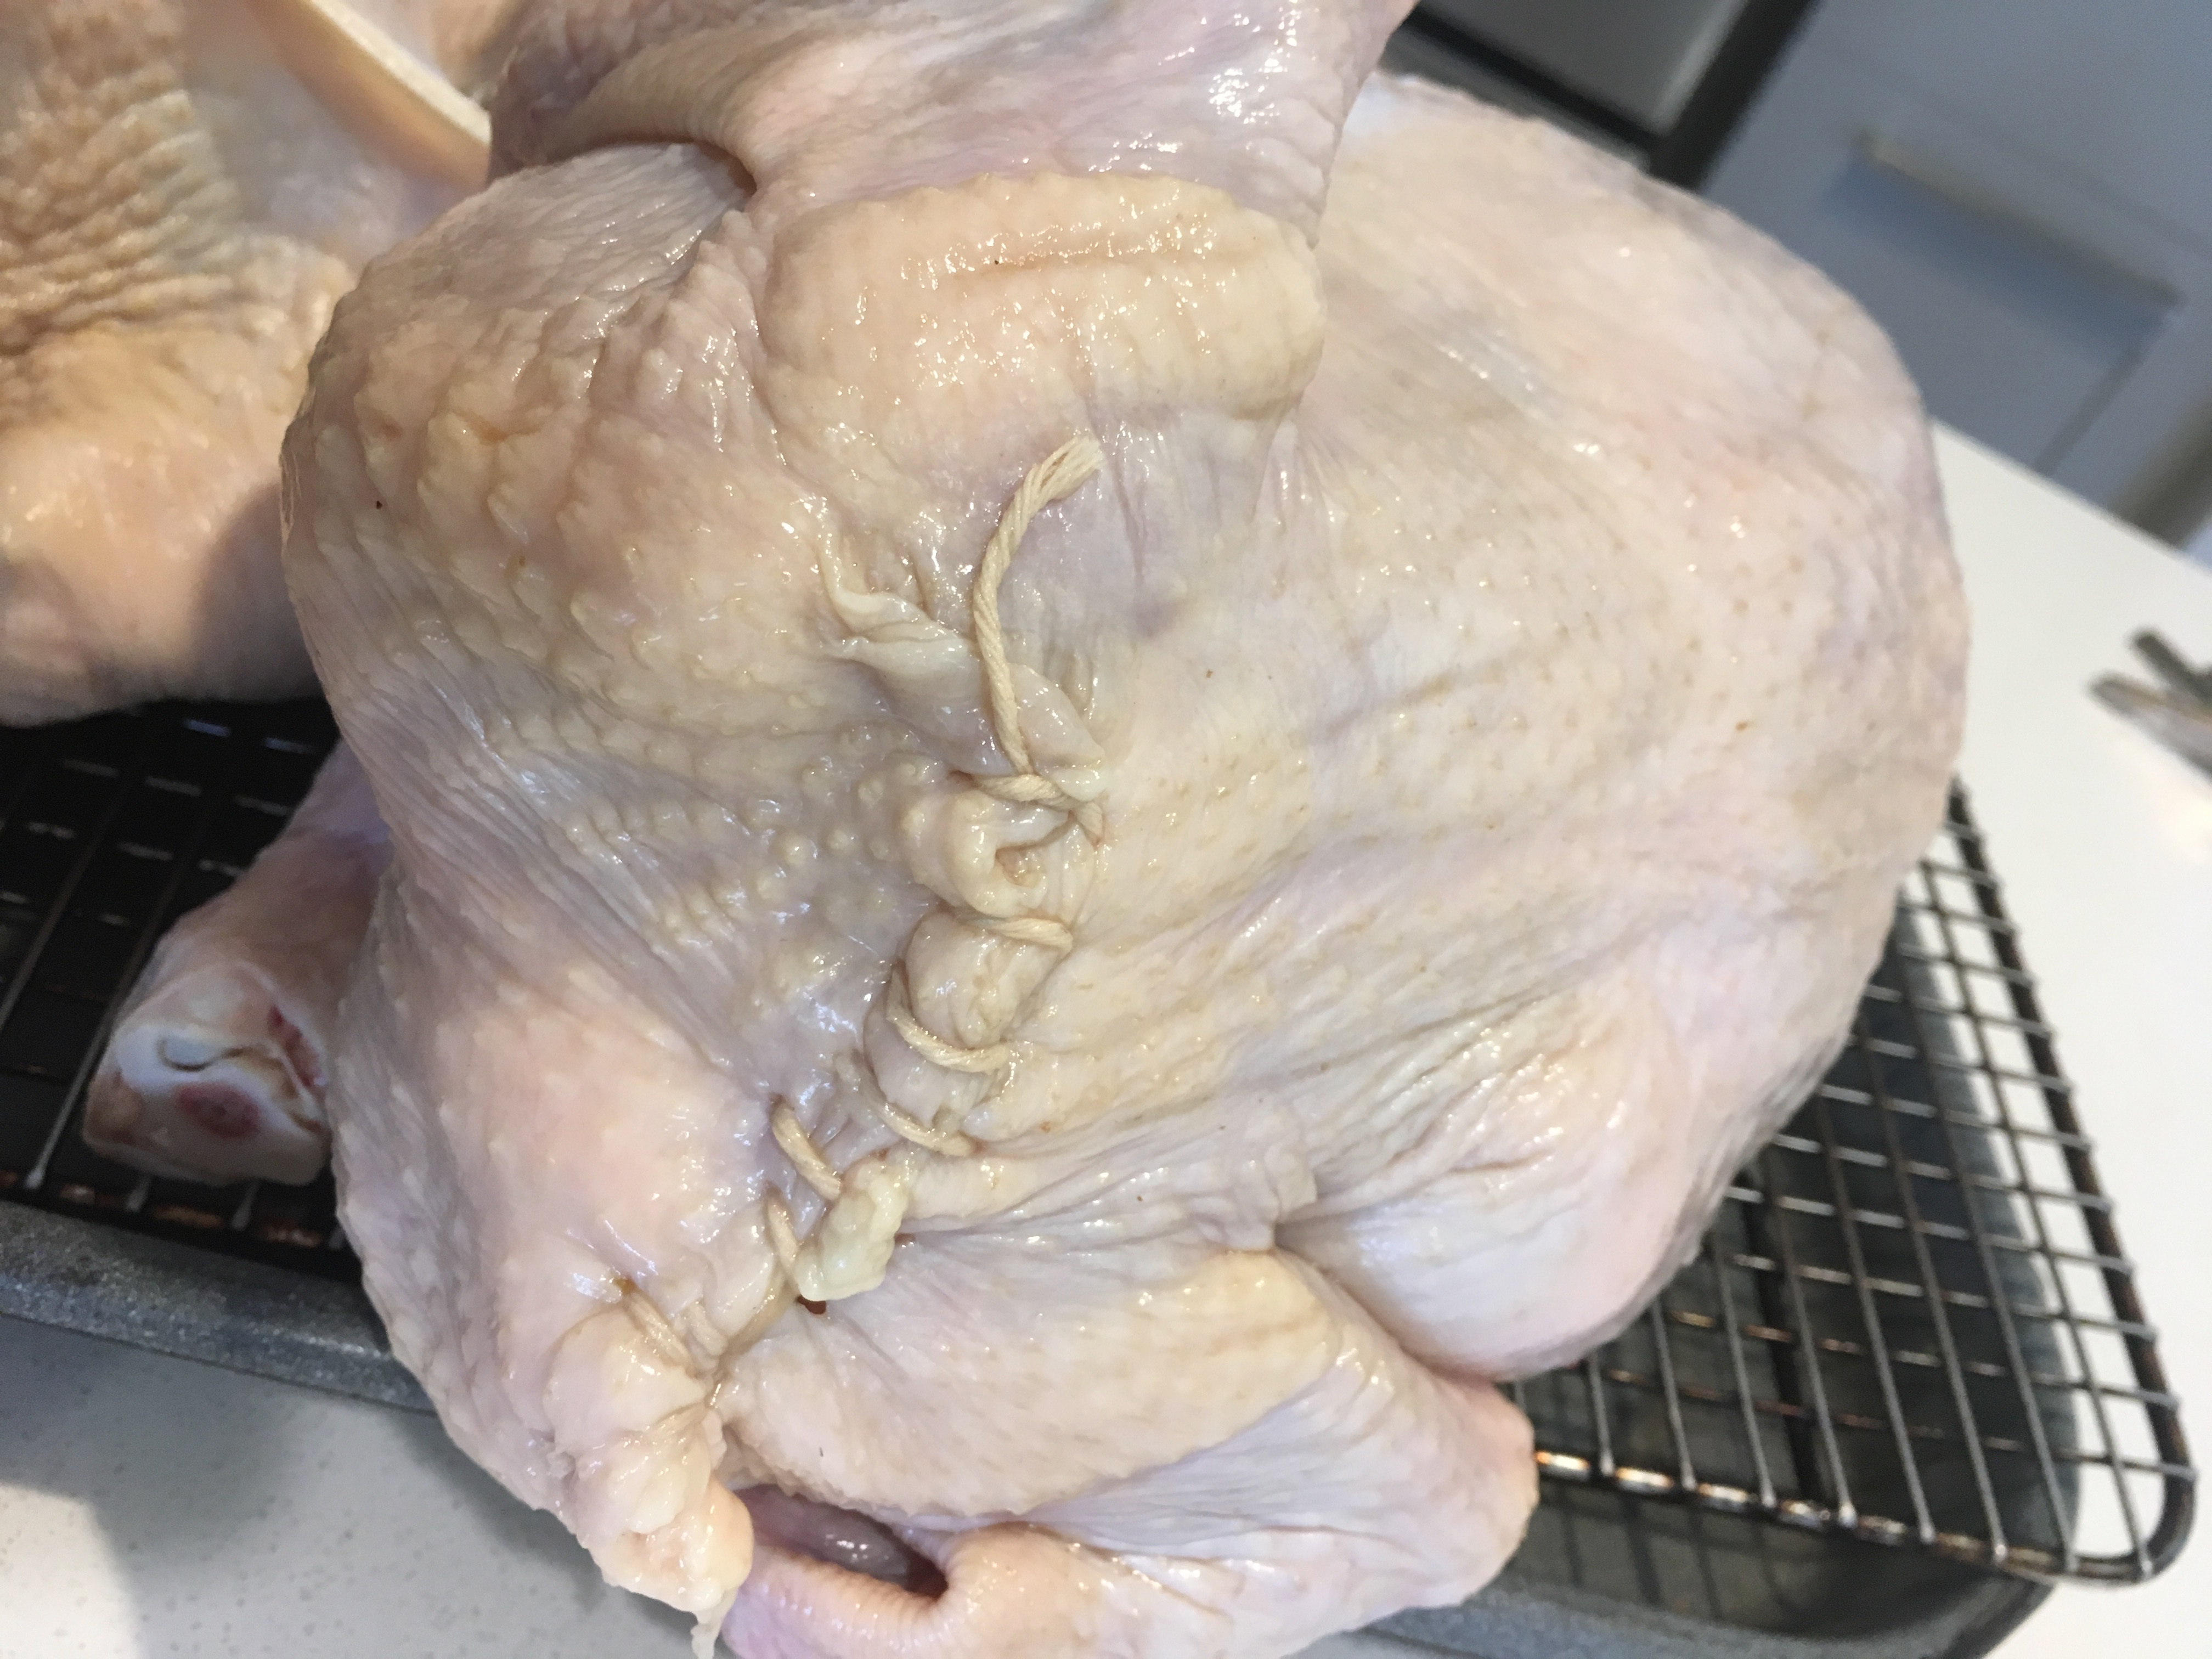
\includegraphics[width=0.25\textwidth]{\imageDir/\fileName/IMG_3218.jpg} &
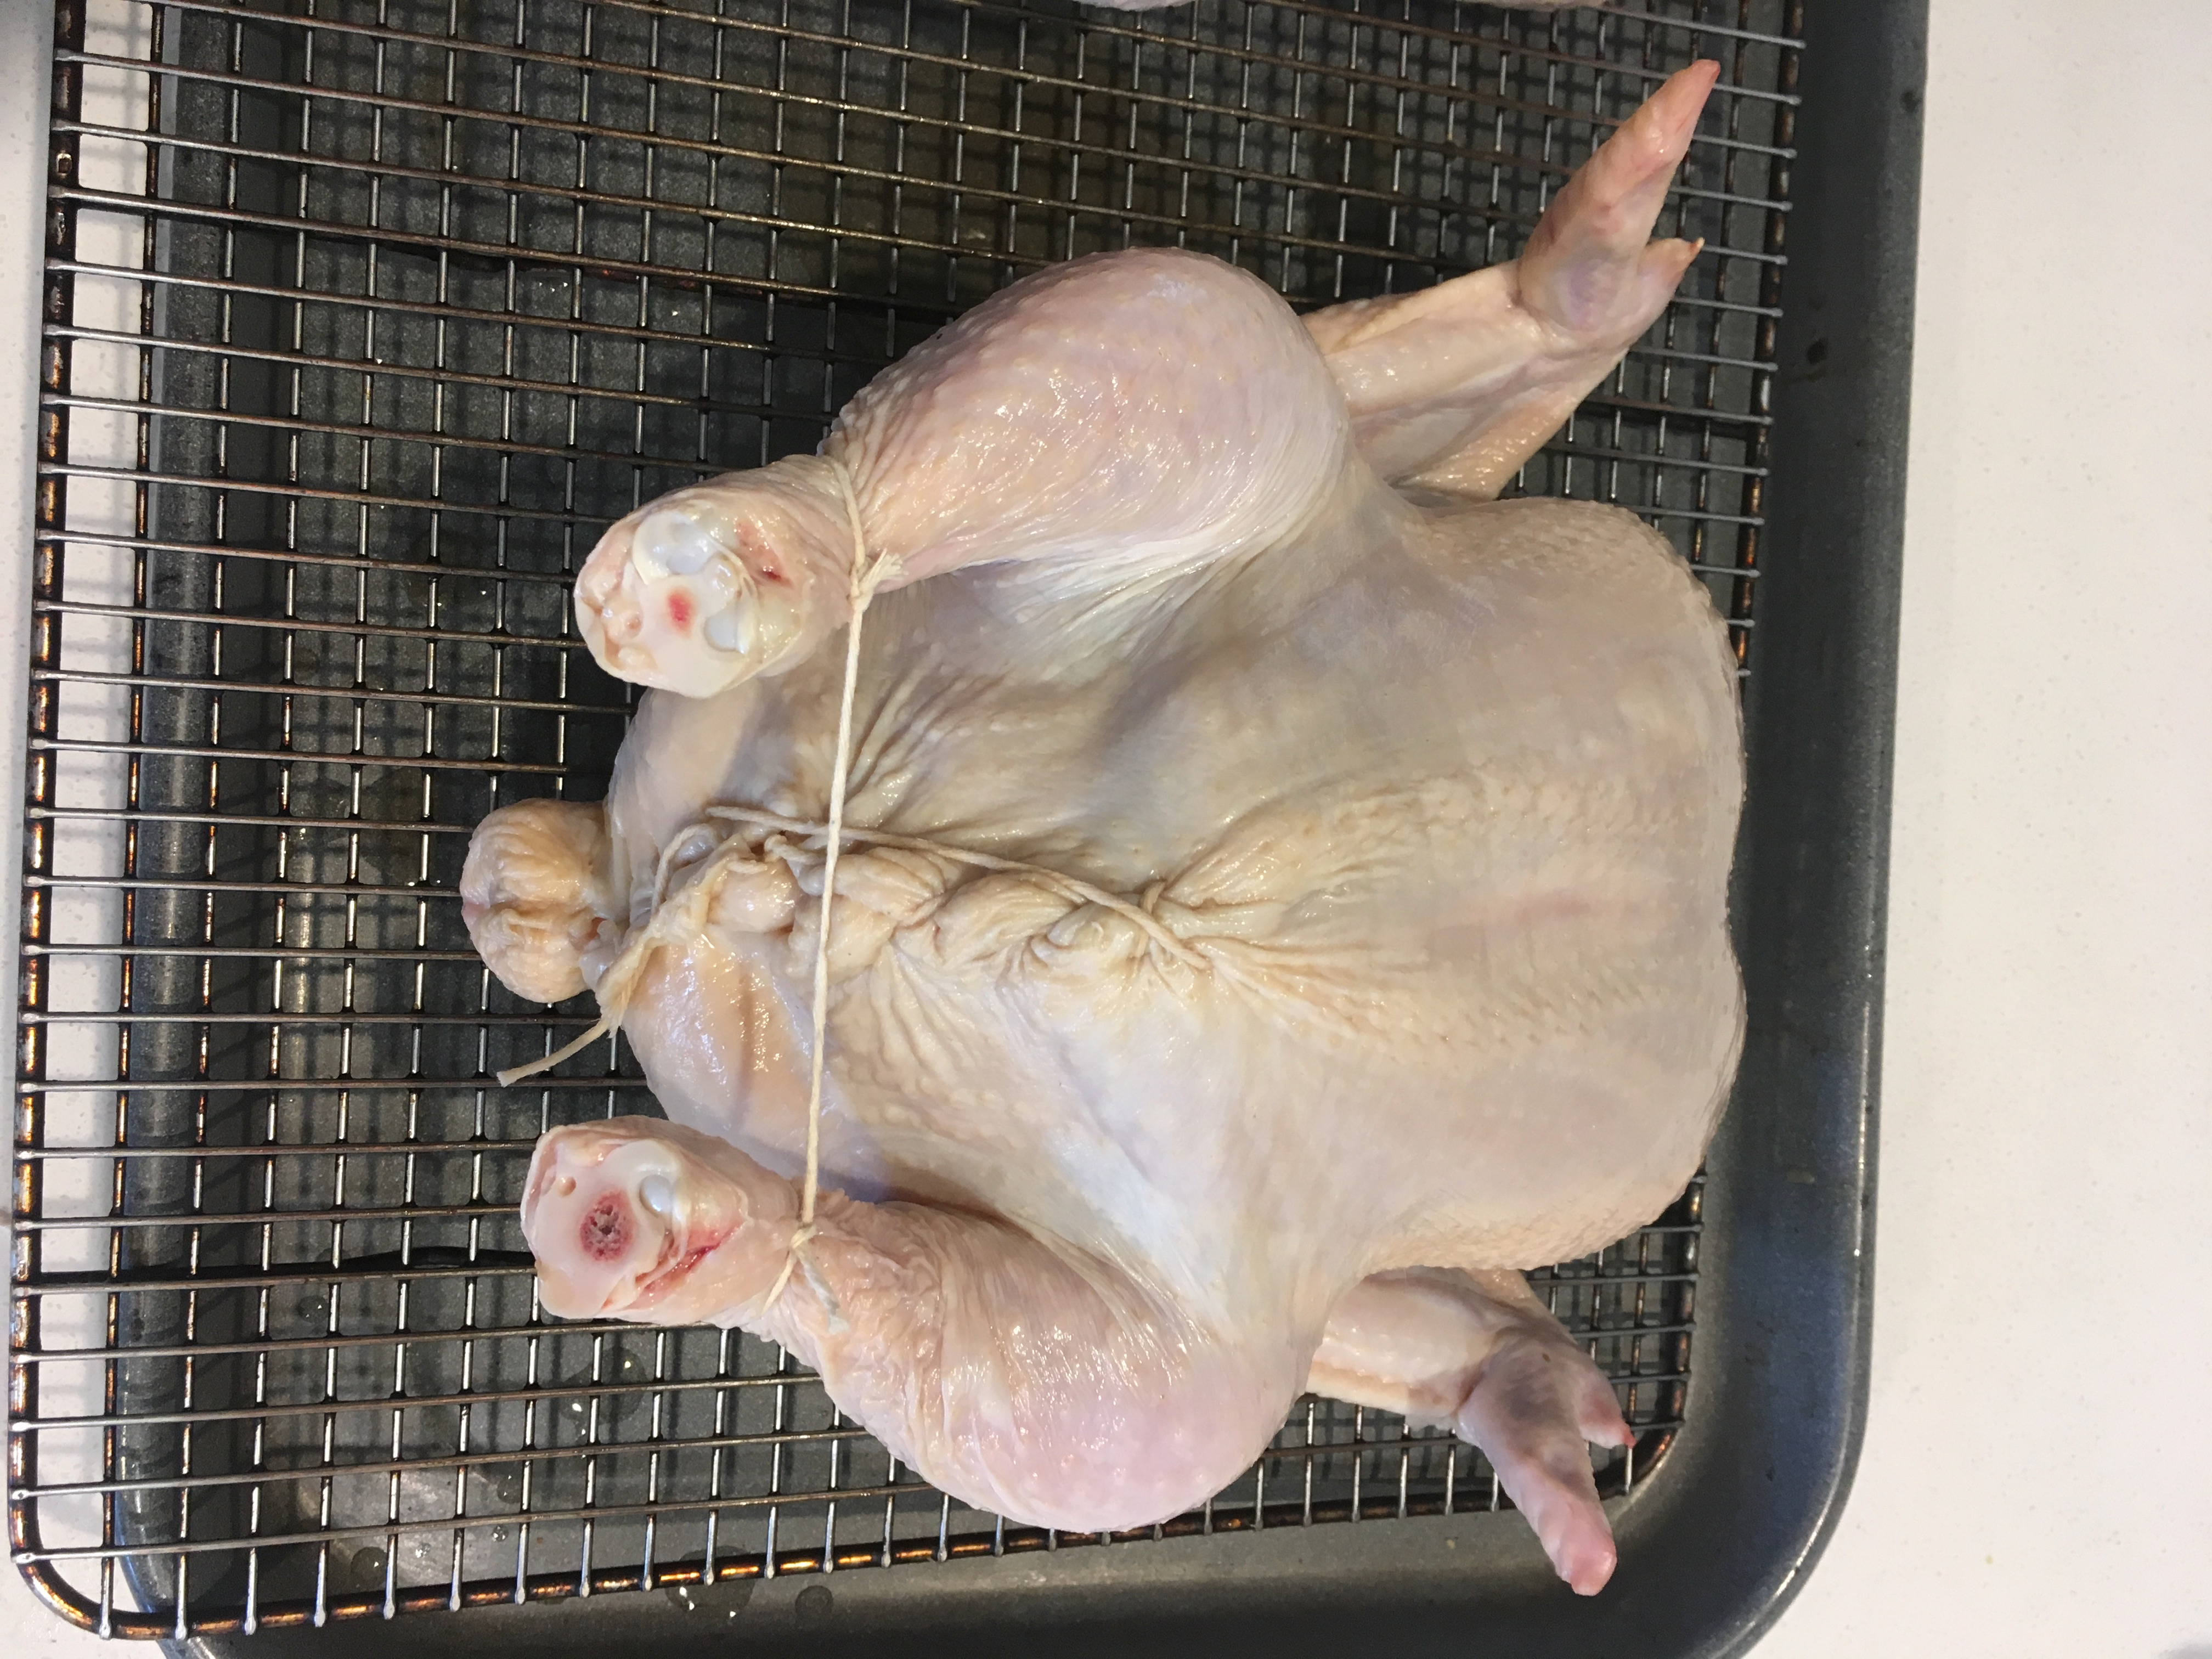
\includegraphics[width=0.25\textwidth]{\imageDir/\fileName/IMG_3219.jpg} \\
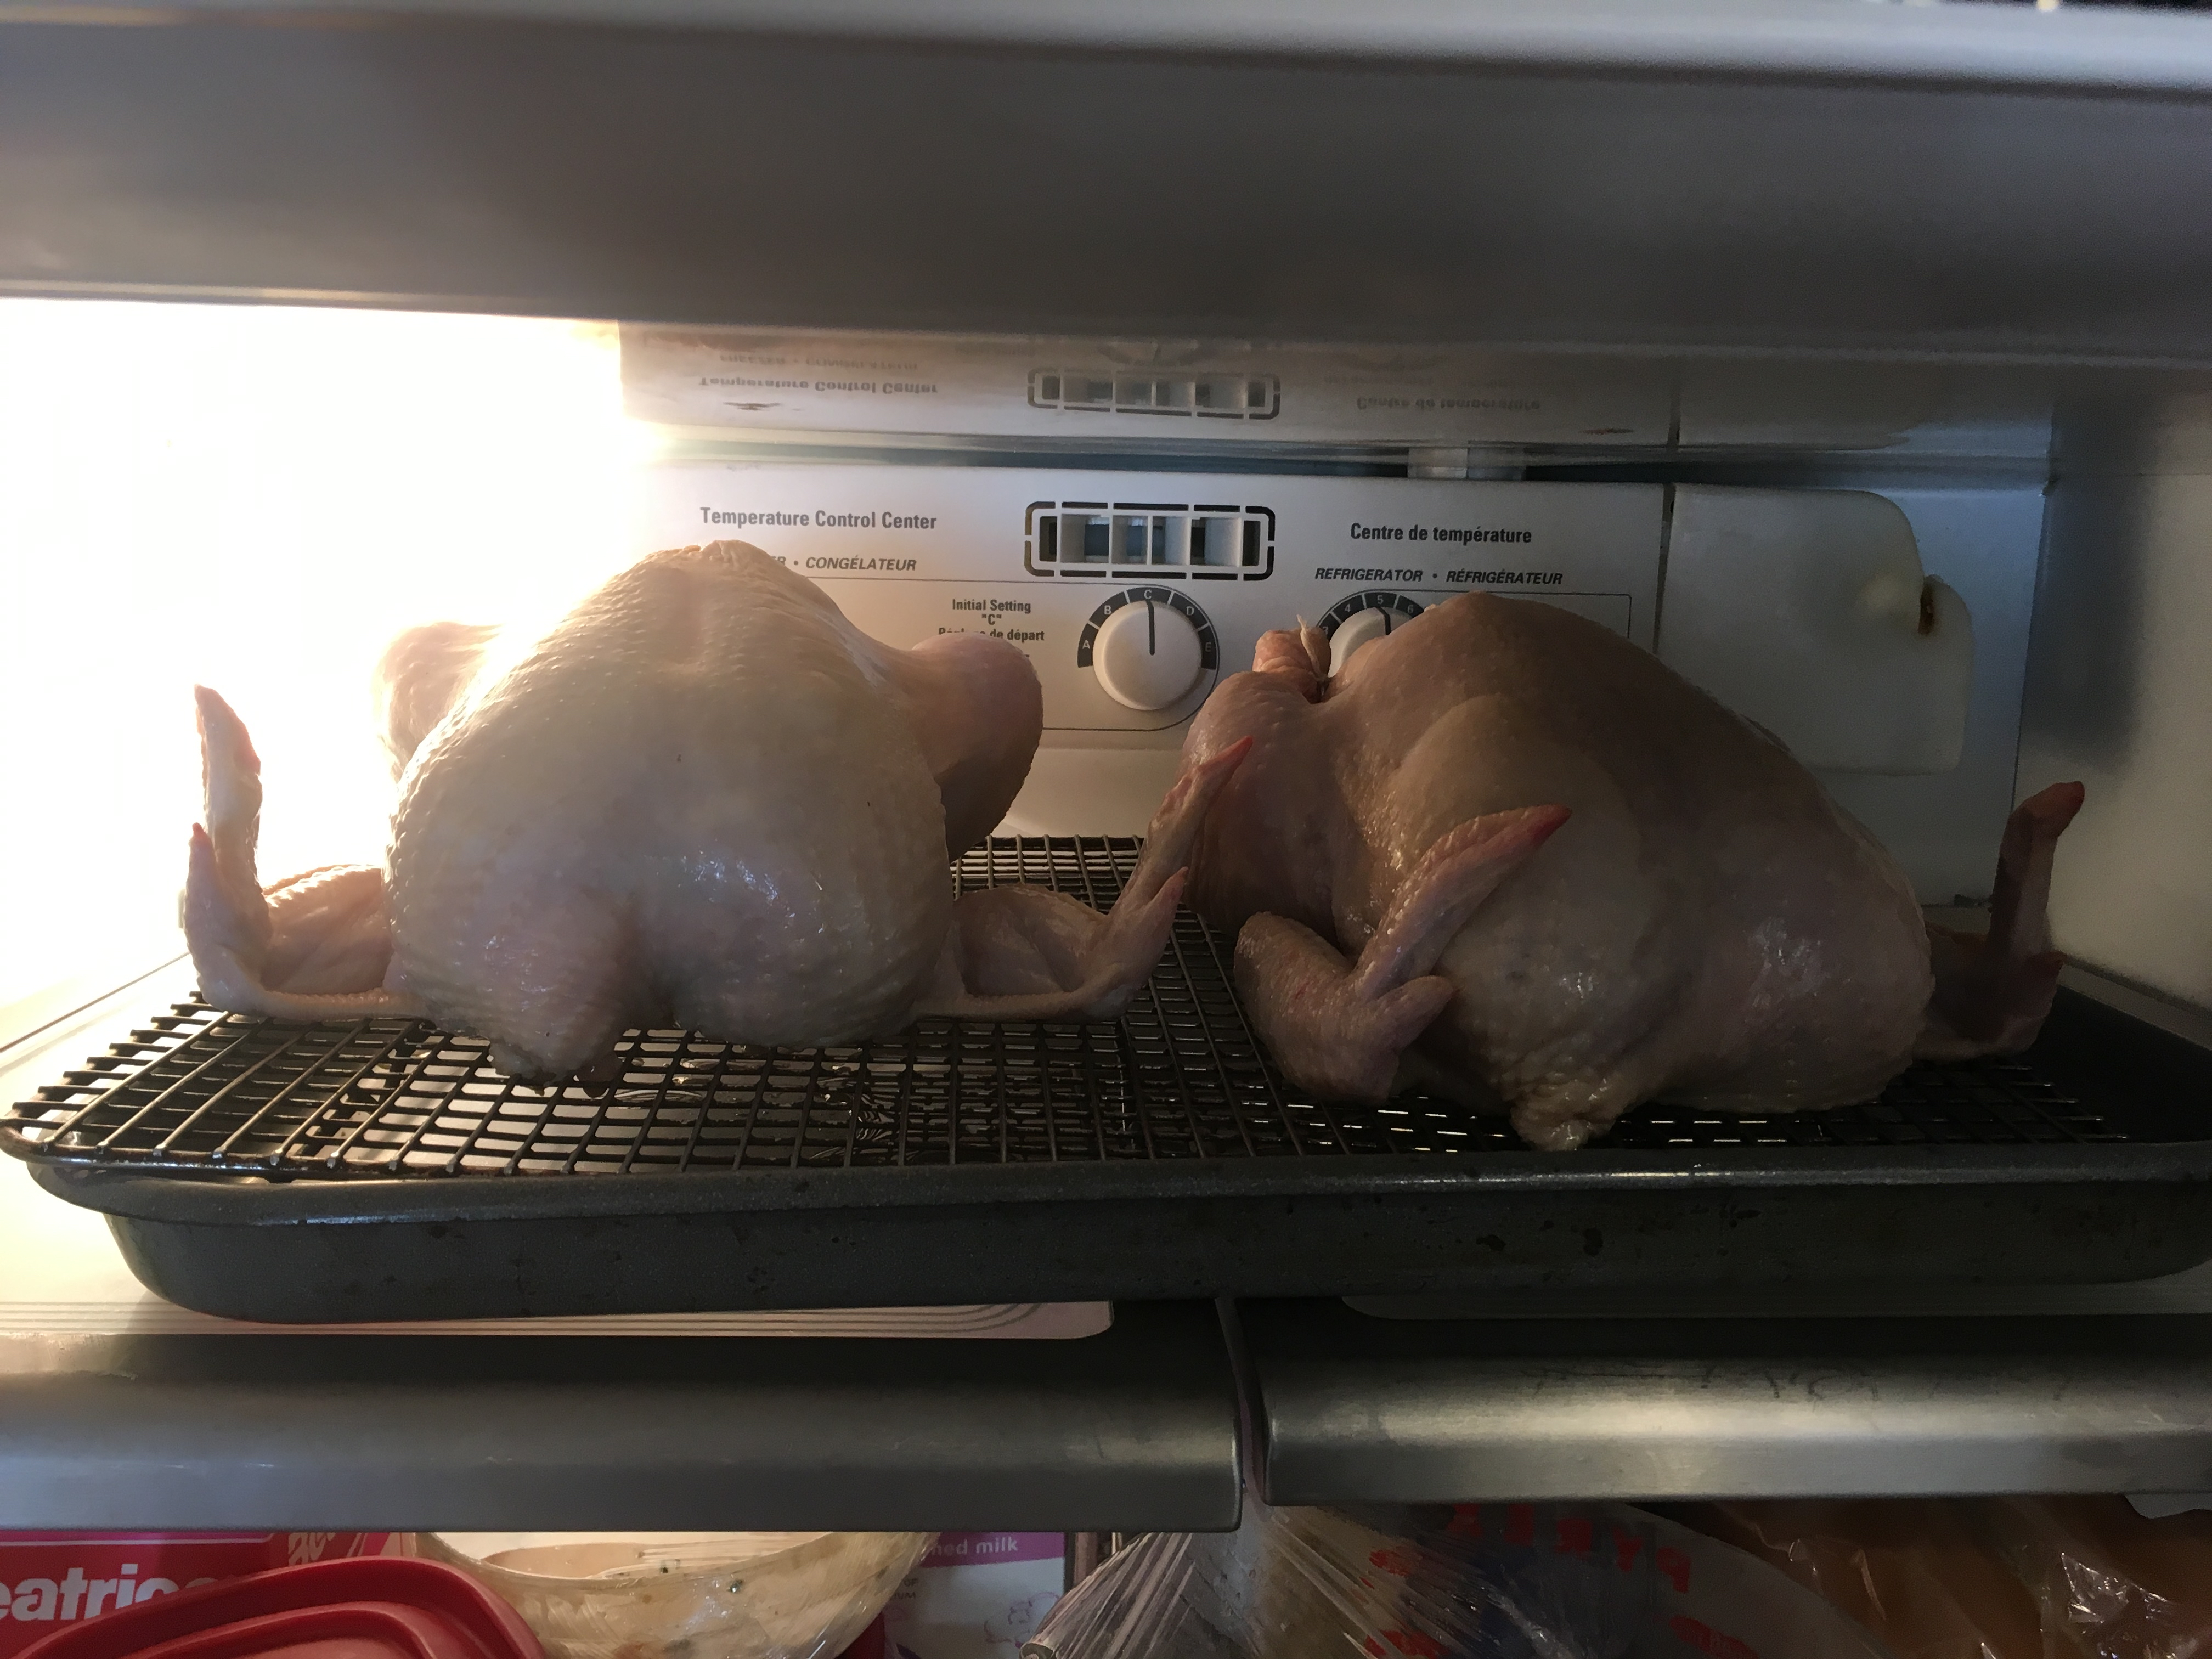
\includegraphics[width=0.25\textwidth]{\imageDir/\fileName/IMG_3220.jpg} &
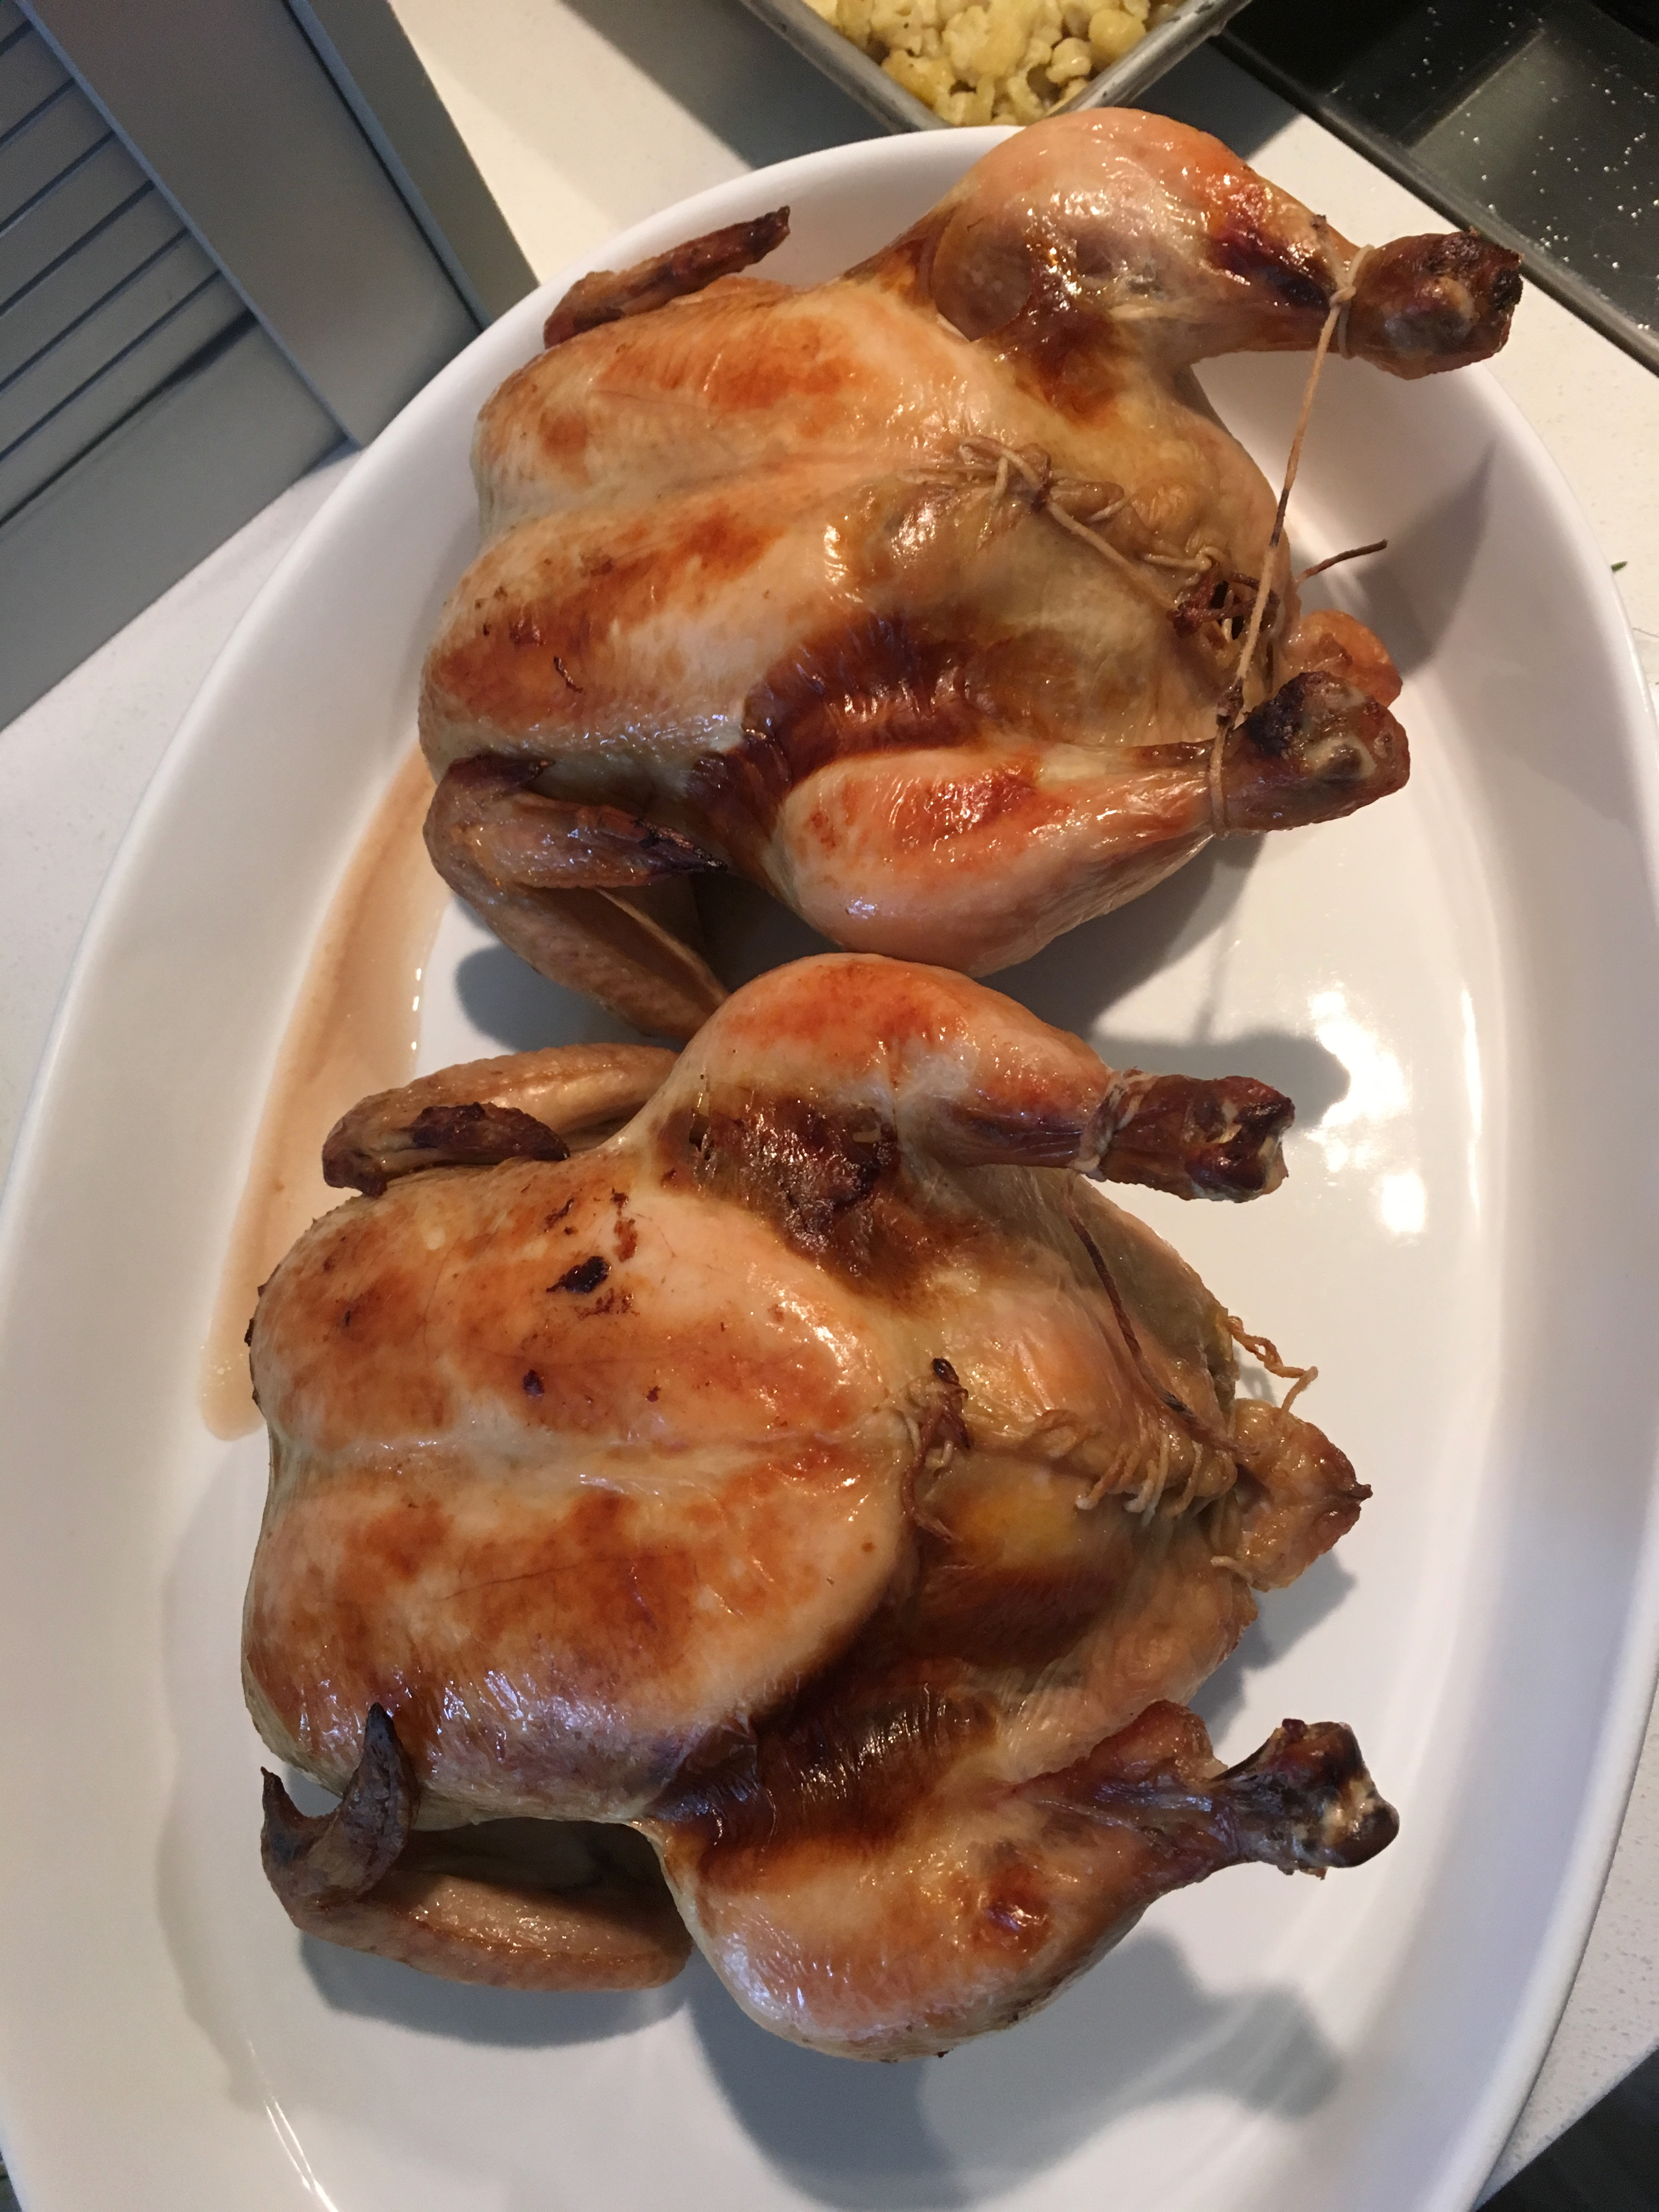
\includegraphics[width=0.25\textwidth]{\imageDir/\fileName/IMG_3228.jpg} \\
\end{tabular}
\end{table}

\end{document}



